The goal of this thesis is to model applications that rely on the Portals API
for their network transport. Although these applications are written using
high-level communication libraries, we also want to take model low-level
properties of the BXI hardware. This leads us to design a simulator that is
abstract enough to be able to scale to hundreds of simulated processes, but
which also features a model of the BXI NIC that is realistic enough to model the
most significant optimizations of the hardware.

This chapter presents the simulator that we designed, S4BXI by focusing on the
low-level model, whereas Chapter~\ref{chap:high_level} will give more details on
how it integrates with high-level APIs such as MPI. S4BXI is based on SimGrid,
and as such it is a Discrete Event Simulator (DES) based on a cooperative actor
model. It models the Portals~4 API, and as such it is by design a good model for
BXI NICs, which implement this API in hardware. It is made in C/C++ from around
9 thousand lines of code\footnote{Counted using cloc:
\url{https://github.com/AlDanial/cloc}}. Finally, it is open-source under LGPLv2
license, and all the relevant links (source code, publications, related tools,
etc.) can be found at \url{https://s4bxi.julien-emmanuel.com}.

We will start by describing how the real-world hardware is
modeled using SimGrid's platform, as well as how we instantiate Actors on this
platform, and then we will detail some technical aspects of our Portals
implementation. Finally, we will present some validation experiments at a low
level before moving on to higher-level experiments in the next chapter.

\section{Platform model}

As introduced in Chapter~\ref{chap:biblio_simu}, SimGrid platforms are composed
of Hosts, that represent simulated hardware, and Links, which represent cables
(or buses). SimGrid allows any combination of Hosts and Links, but for the
purpose of our simulators we add a few constraints on this representation.

\subsubsection{Host types} 

In SimGrid, Hosts are supposed to be able to represent whole machines, and
SimGrid natively allows to configure a Host as multicore (a virtual Host in the
model can have several virtual cores). SimGrid does not have a fine model of
scheduler inside each Host, and it does not model each core independently, which
means that in practice, in the case of a multicore Host, every computation phase
is evenly distributed across all cores.

In our case this proved to be problematic, as we wanted to be able to assign
specific tasks to specific (virtual) cores, instead of having each computation
phase distributed across all cores. For this reason, in S4BXI we use Hosts not
to model full machines, but instead we define two types of Hosts, which
represent hardware at a finer granularity: we have Hosts that represent a single
CPU core, and Hosts that represent a NIC. This means that in practice, in our
model each physical machine is represented by $N + 1$ virtual Hosts, where $N$
is the number of cores in the CPU.

\subsubsection{Link types} To connect these Hosts together, we have two types of
Links: PCI Links and BXI Links. PCI Links model the PCIe bus inside each
machine, which connects the NIC to the rest of the machine. This link is
important because it is typically not modeled by other flow-level simulators, in
particular SMPI, which usually models a whole machine with a single Host. We
decided to do it because as interconnection networks get faster and faster, the
transfer times across the PCI bus is of the same order of magnitude as network
transfer times, which means that congestion on the PCI bus can happen and have
an impact on the speed of inter-node communications. The second type of Links is
the more traditional network cables that connect NICs to switches, and switches
together.

\begin{figure}[!ht]
    \centering
    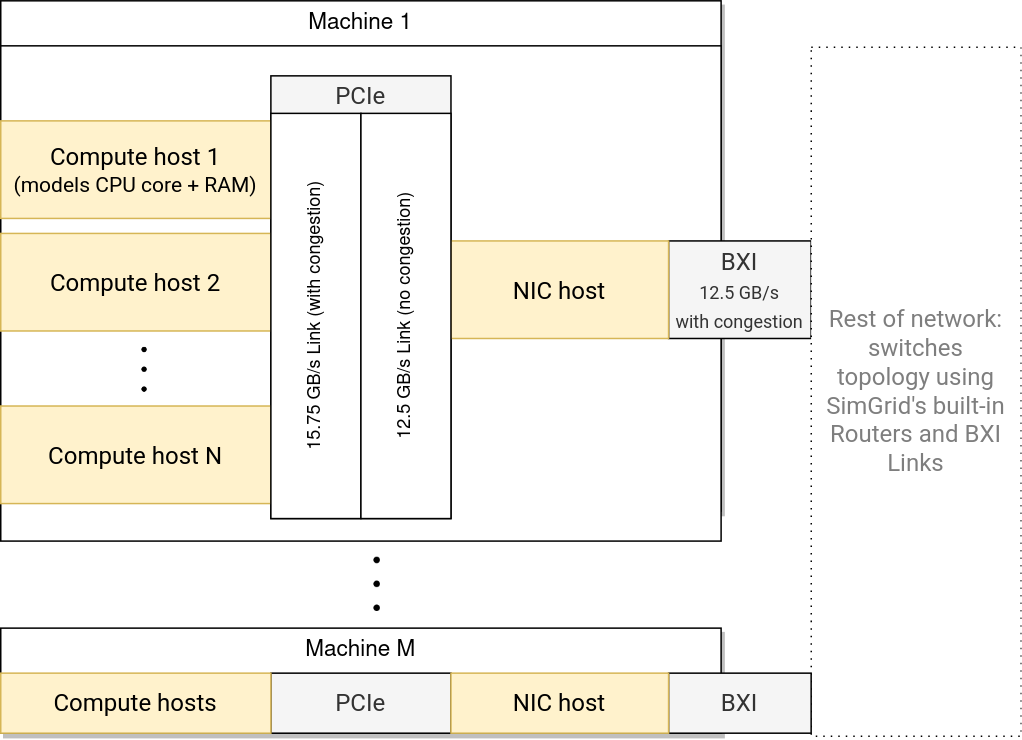
\includegraphics[width=0.8\textwidth]{4_portals/hosts_links.png}
    \caption{Platform model in S4BXI}
    \label{fig:4_portals:Hosts_Links}
\end{figure}

One of the difficulties resides in the model of the PCI bus: while third
generation PCIe x16 networks have a maximum theoretical bandwidth of 15.75 GB/s,
most of our transfers (especially the transfers of consequent size) are going to
flow from the PCI bus directly onto the BXI cable (which has a maximum bandwidth
of 12.5 GB/s), with minimal processing in the middle. In real life this is
handled with packetisation on each side of the NIC (across the PCI bus and then
across the BXI cable), but because we use a flow model that operates at
message-level, we cannot implement this level of granularity without losing a lot
of performance. While we cannot model a total maximum bandwidth of 15.75 GB/s and
a per-message bandwidth of 12.5 GB/s in a single Link in SimGrid, we can model
this behavior using two Links that each transfer has to go through: a 12.5 GB/s
Link on which congestion is not considered, which limits the speed of each
individual transfer, and a 15.75 GB/s Link on which congestion is considered,
which limits the speed of all simultaneous transfers across the bus at any given
time. We are allowed to connect these two Links back to back in simulation, even
though it does not correspond to what can be done in real life. Indeed, SimGrid
is very permissive in the description of platforms: every Host and Link has a
Netpoint (in SimGrid vocabulary), which can be connected to any other Netpoint
regardless of the type of hardware it is bound to, so it effectively allows
users to connect Links together.

It is worth noting that there is no particular model for switches: indeed, we
use native Router components provided by SimGrid to represent BXI switches, but
even these components are just syntactic sugar to represent a Host with no
Actors. These Routers work even though they do not implement any behavior,
because the routing logic across the cluster (i.e. the set of Links to be used
when communicating between two Hosts) is not performed at a high-level by
Actors, but it is implemented at a low-level in the SURF layer of SimGrid. While
making a more detailed model of switches at S4U-level using Actors would be an
interesting subject of study, we chose to use the defaults routing algorithms
offered by SimGrid in SURF because their fat-tree routing is faithful enough to
what happens in real-world BXI fat-trees for our needs.

The platform model that results from our Links and Hosts is depicted on
Figure~\ref{fig:4_portals:Hosts_Links}, with a focus on one machine composed of
$N$ CPU cores.

\section{Actor placement}

Along with the platform description, a simulation needs to know which Actors to
deploy on the simulated Hosts, which is done through a ``deployment'' in
SimGrid. Similarly to the platform description, this can be done either
statically in XML or dynamically in C++. Throughout this thesis we used a static
XML deployment, since it is more concise than platform files, and therefore does
not suffer the same performance issues (even though in some situations S4BXI may
spawn a short-lived Actor to delay a specific task). Since the different types
of Actors to be deployed are the same in each simulation, and only numerical
parameters change (number of process to be deployed, number of nodes to be used,
etc.), we made tools to automate the process of generating deployment
files\footnote{\url{https://framagit.org/s4bxi/s4bxi-config-generator}}.

In order to implement the Portals API on top of the simulated hardware described
earlier, S4BXI provides several types of Actors, each of which correspond to a
different part of the communication logic. Their placement is represented on
Figure~\ref{fig:4_portals:actor_placement} and will be detailed in the next
sections.

\begin{figure}[!ht]
    \centering
    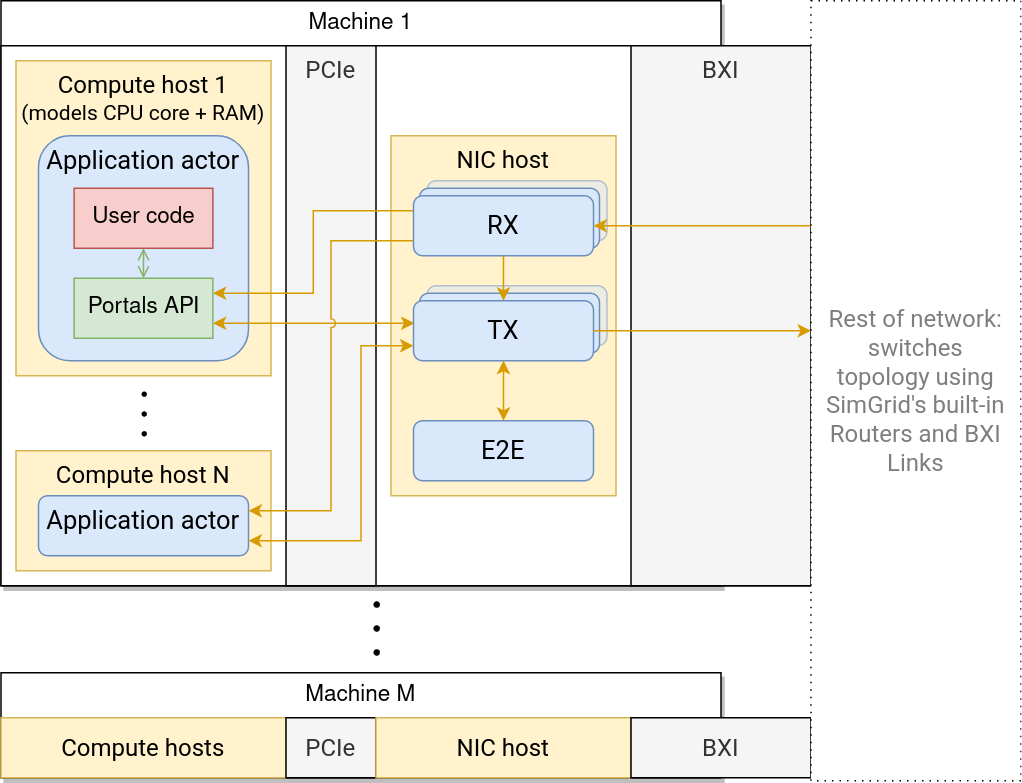
\includegraphics[width=0.8\textwidth]{4_portals/actor_placement.png}
    \caption{Actor placement in S4BXI}
    \label{fig:4_portals:actor_placement}
\end{figure}

\subsection{On-NIC Actors}

Since the Portals API is implemented in hardware by the BXI NIC, most of the
Portals implementation is done through three types of Actors that are
instantiated on the ``NIC Host'' of each machine in our platform:

\subsubsection{TX Actor}

TX Actors model the ``transmission'' logic of the NIC. This means listening to
command queues, processing message requests by doing any Direct Memory Access
(DMA) and generating any event that might be required, and finally sending
messages on the BXI Link to the rest of the network (through SimGrid's Mailbox
system). While the simulation works with only one TX Actor per NIC, users of
S4BXI can choose to instantiate several, either to model parallel processing
capabilities of the NIC, or to model different types of traffic. In BXI this
last feature corresponds to the Virtual Networks that were presented in
Section~\ref{subsubsec:2_context_hpc:VNs}.

\subsubsection{RX Actor}
\label{subsubsec:4_portals:RX}

RX Actors model the ``receive'' logic of the NIC. To do this they listen to
SimGrid Mailboxes, of which they are the permanent receiver (so that incoming
messages can keep flowing in even if no Actor is available to process them yet,
as described in Section~\ref{sec:3_related_work_simu:simgrid}). Then these
actors process the request depending on its type, applying any Atomic operation,
etc., and finally if an ACK or a Response is to be sent back it will be
forwarded to the corresponding TX command queue (either \textit{compute} or
\textit{service}). Similarly to TX Actors, RX Actors can be instantiated several
times to model different VNs, or parallel processing capabilities of the
hardware. For example, BXI NICs typically have four independent
Application-Specific Instruction set Processors (ASIP) for this purpose, which
are called List Management Engines (LME).

\subsubsection{E2E Actor}

E2E Actors model the End-to-End reliability logic of the NIC which was described
in Section~\ref{subsubsec:2_context_hpc:E2E}. Since our simulator implements a
flow model at message-level, it cannot model the CRC processing (encoding at
sender, verification at receiver), since it is performed on each packet, but it
models completely the timeout mechanism that is implemented in BXI, to
retransmit messages which did not get acknowledged on time. The parameters
(number of retransmissions and delay before retransmitting) are tunable using
environment variables (\inline{S4BXI_MAX_RETRIES} and
\inline{RETRY_TIMEOUT} respectively). In S4BXI, the E2E Actor of each machine
receives a copy of each message that is issued by TX. The only exception is for
BXI ACKs: in order not to have an infinite loop of acknowledgements (similar to
the Two Generals'
Problem\footnote{\url{https://en.wikipedia.org/wiki/Two_Generals_Problem}}),
these messages cannot have a further level of ACK, and they are therefore
delivered unreliably. For each message, the E2E Actor then sleeps until the
delay for retransmission is met. It then checks if an RX Actor has marked the
message as ``acknowledged'' or not, and either drops the message if it is the
case, or sends it back to the TX command queue for retransmission if the message
seems to have been lost. This logic is represented on
Figure~\ref{fig:4_portals:e2e_logic}: in this example only the first message
sent is acknowledged in time, so the second one needs to be retransmitted.

\begin{figure}[!ht]
    \centering
    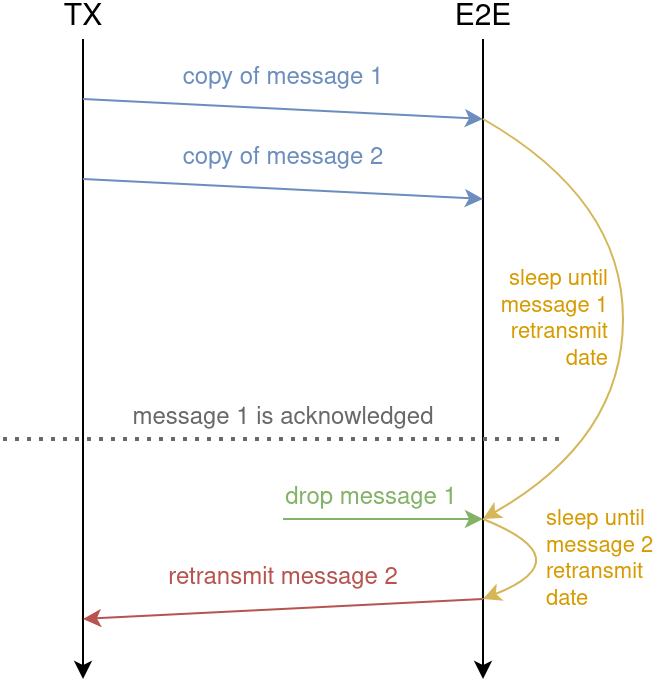
\includegraphics[width=0.6\textwidth]{4_portals/E2E_seq.png}
    \caption{E2E logic in S4BXI}
    \label{fig:4_portals:e2e_logic}
\end{figure}

It is important to note that although several RX and TX Actors can be
instantiated, every machine only requires one E2E Actor. This is because the
delay before retransmitting a message is constant in BXI (as it is a parameter
of the BXI kernel module), and therefore if messages need to be retransmitted it
will always be in the same order that they are received in by the E2E Actor.
This means that this Actor can safely sleep until the next retransmission date
when it processes a message, because even if another one is created in the
meantime its retransmission date will necessarily occur later. Additionally, we
can use a single ``First In, First Out'' (FIFO) data structure for all
communications between TX Actors and the E2E Actors (in which TX Actors writes
messages, which are read by the E2E Actor).

\subsection{Actors on CPU cores}
\label{subsec:4_portals:UserAppActors}

While the Actors instantiated on the NIC have a fixed behavior, Actors deployed
on the simulated CPU cores must be more flexible in order to model any user
application (as long as it uses the Portals API as its communication layer of
course). This is done in a way that is strongly inspired by SMPI: S4BXI requires
the user application to be compiled as a shared library, which allows the
simulator to use the \inline{dlopen} and \inline{dlsym} C functions to
load the \inline{main} function from the program and run it in simulation.
Since SimGrid uses cooperatives Actors, the user application simply yields
automatically when any network operation is performed, through the Portals API
which links with the implementation in S4BXI instead of a real-world one.

\section{Portals model}

\subsection{Representation in S4BXI}

In S4BXI, data exchanges are modeled using different Mailboxes, depicted in
Figure~\ref{fig:4_portals:s4bxi_mailboxes}. We can see that the event system
translates to a variable number of mailboxes (one for each EQ) that are created
through allocations by the user code (\inline{PtEQAlloc} for EQs for example),
and can then be queried through the Portals API. The mailboxes on the NIC do not
directly map to Portals data structure, instead they are an approximate model of
the hardware pipeline inside BXI NICs. We did not go for a faithful
representation here, because the real-word components of the NIC are very
complex, feature many more queues, and manipulate data at a different
granularity in different places (for example packet size on the network is 72
bytes, while transfers across a PCI bus can range between 128 and 4096 bytes of
packet size), whereas our simulator models traffic at message level, and
therefore is not suited to model individual packets in the NIC. This design
costs some accuracy, but greatly improves the performance of S4BXI.

In our model, TX Actors share \portalsAbbr{Commands Queues}{CQ}, one for each
Virtual Network that is used by the simulation's deployment (since inside each
VN operations must be strictly ordered according to the Portals's
specification). They wait for commands from other Actors in an infinite loop and
process them sequentially. These command queues are not directly Mailboxes: we
added a layer of abstraction on top of it that we will call ``S4BXI Queue''.
These queues mimic the Mailbox interface, but they provide two implementations:
they can either simply map to a Mailbox internally, or use a more performant
implementation based on a C++ \inline{std::queue} to store entries and a
\inline{simgrid::s4u::Semaphore} to allow processes to wait for a piece of data
to be available (a standard C++ semaphore cannot be used because it needs to be
blocking in the simulated world). This allows our queues to either model the
time it takes to transfer data to them (using the Mailbox system), or to make
operations instantaneous, which is often less accurate but will slightly improve
the performance of the simulator. Similarly, RX Actors also poll on Mailboxes,
one per VN, but which contain the incoming messages from the network. These
Actors implement the processing of these messages, including the matching logic
of MEs, any memory operation that might be required, and if a response is
needed, it is created in the RX Actor and forwarded to TX Actors through the
corresponding S4BXI Queue. Finally, the E2E Actor has its own S4BXI Queue, which
receives a copy of each message that TX Actors send on the network, except for
BXI ACKs which do not have their own acknowledgement.

\begin{figure}[!ht]
    \centering
    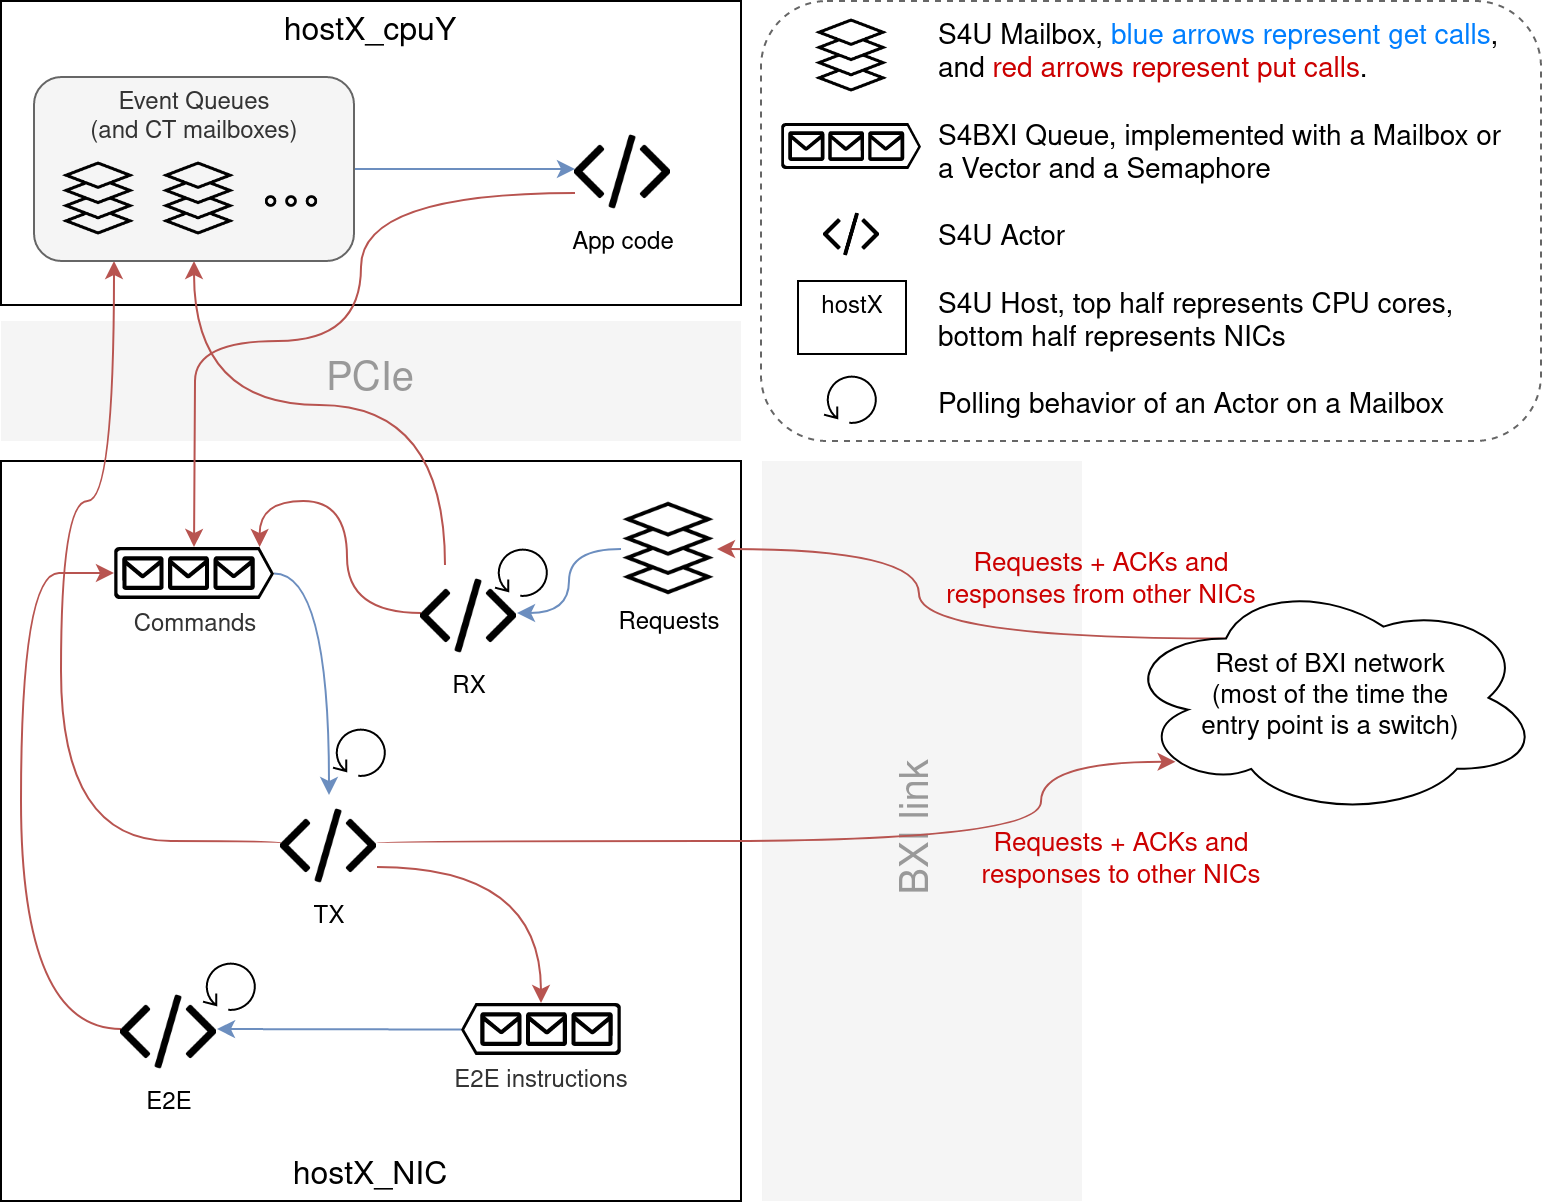
\includegraphics[width=1\textwidth]{4_portals/s4bxi_mailboxes.png}
    \caption{Mailboxe usage in S4BXI}
    \label{fig:4_portals:s4bxi_mailboxes}
\end{figure}

\subsection{Tuning for the BXI interconnect}

While Portals is a good specification for the API that should be exposed to
users, at the lowest level significant freedom is left to the implementation.
This results in many low-level design choices that need to be made in order to
run this API on real-world hardware. Several of these characteristics cannot be
modeled directly in S4BXI, because they are implemented at flit-level in BXI
hardware. This is the case of low-level flow control for example, which is
achieved using a credit-based mechanism in the real-world hardware. In this
section we will present the specific properties of BXI which are modeled in
S4BXI, because they operate at a level of granularity that is coherent with our
flow model.

\subsubsection{Virtual Networks}

Virtual Networks in BXI were presented in
Section~\ref{subsubsec:2_context_hpc:VNs}. They are fully modeled in S4BXI, by
assigning a VN number (from zero to three) to TX and RX Actors. Internally this
will result in the creation of several independent command queues that will
receive requests for TX actors, and independent Mailboxes that will receive
incoming messages for RX Actors (only one of each is represented on
Figure~\ref{fig:4_portals:s4bxi_mailboxes}). The difference between SERVICE and
COMPUTE VNs is not the most important in simulation, since S4BXI does not
support simulating any code that would typically run in SERVICE mode (such as a
NFS). On the other hand, the difference between REQUEST and RESPONSE VNs is
interesting to model so that ACKs and replies can progress independently from
requests.

\subsubsection{Command Queue depth}

\begin{figure}[!ht]
    \centering
    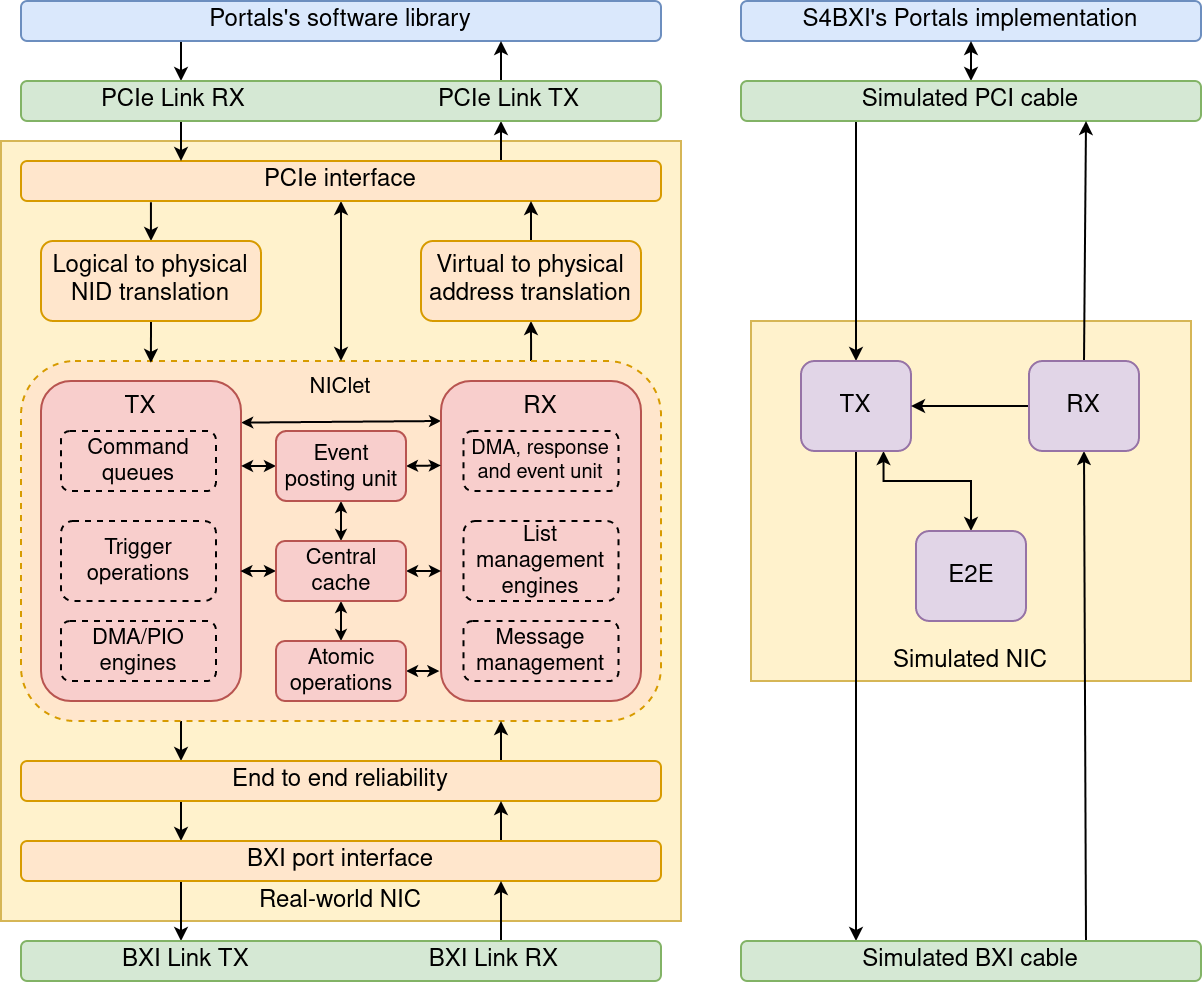
\includegraphics[width=0.9\textwidth]{4_portals/pipeline_comparison.png}
    \caption{Internal pipeline of BXI NICs compared to S4BXI's implementation}
    \label{fig:4_portals:pipeline_comparison}
\end{figure}

Even though there is no particular restriction in Portals itself, in the real
world limitations of the hardware imply that queues have a finite size, and
therefore applications can only buffer a limited number of commands on the NIC
before its command queues run out of space. This phenomenon is modeled in S4BXI,
but in a slightly different way than  in the real-world hardware: as explained
earlier, the real-world NIC features many components that communicate together
through internal queues. This means that the processing of commands goes through
a pipeline, as shown in Figure~\ref{fig:4_portals:pipeline_comparison}. Thanks
to this property, several commands can be in the pipeline at the same time (in
different stages), which gives the software an illusion of parallel processing
(although the vast majority of hardware components are strictly sequential). It
also means that the first component in the pipeline is going to consume commands
faster than we would expect in simulation: in S4BXI the whole processing of a
command is implemented as a single sequential block of code (usually in the TX
Actor's logic), which means that the internal NIC queues that operate on various
packet sizes are not modeled in detail. Because of this, even though we know
that the queues between the CPU and the NIC have 16 entries in them, we need to
increase the queues' size in simulation, in order to account for the depth of
the whole pipeline. From our experimental tests we have determined that a depth
of 89 entries in TX queues in S4BXI give the most accurate result, but it is
important to note that this is only determined empirically, as we do not know in
detail the depth and speed limitations of all intermediate queues inside the
real-world NIC.

\subsubsection{Reusing user buffers}

With Portals, sending data usually triggers two events that are sent by the NIC
to the user application: a SEND event and an ACK event (or REPLY if the targeted
node sends data back, in the case of a FetchAtomic request for example). While
ACK events simply inform the user that the message was successfully delivered
and acknowledged, the SEND event is here to inform the user that the buffer from
which data was sent can be re-used safely. What this last part means is
different depending on the size of the payload: for large messages, the SEND
event will be triggered at the same time as the corresponding ACK, because until
the message is fully acknowledged the NIC could still need to access the payload
in main memory in case of a retransmission by the E2E mechanism. For small
messages (up to 64B), on the other hand, the NIC has enough internal cache
storage to keep the full payload in what is called the``E2E context'' of the
message, which means that in the case of a retransmission the main memory will
not be queried. For this reason, the transfer of small messages can be performed
with a significantly lower latency, and achieve high message rates while having
reliable transfers. This mechanism is fully modeled in the TX Actors of S4BXI,
as we will be able to see in the experimental results of
Section~\ref{sec:4_portals:validation}.

\subsection{Streaming data from memory to memory across BXI}

\subsubsection{Real-world behavior}

When sending data (through any request other than \inline{PtlGet} which
performs a remote ``read'' operation), there are three different ways to move
the payload from the memory to the NIC, which depends on the message size and
options:

For the smallest messages, up to 8B for operations with match bits or 16B
without match bits, the payload can be written ``inline'' in the command
directly, since requests do not use the full memory size available for commands,
according to the command format used to communicate with the NIC.

For larger messages, up to 408 or 416B (again depending on match bits), BXI uses
what is called PIO (Programmed I/O). This method requires the CPU to write the
payload (minus the first 8 or 16B) in a small space of ``scratch'' memory on the
NIC, before sending the command with the remaining data (similarly to inline
mode). This allows data to be accessible right away when the NIC processes the
command, but it costs a small amount of time because it requires the CPU to
perform two PCI writes as well as a memory fence between the two (in order to
make sure data is written before the command).

\begin{figure}[!ht]
    \centering
    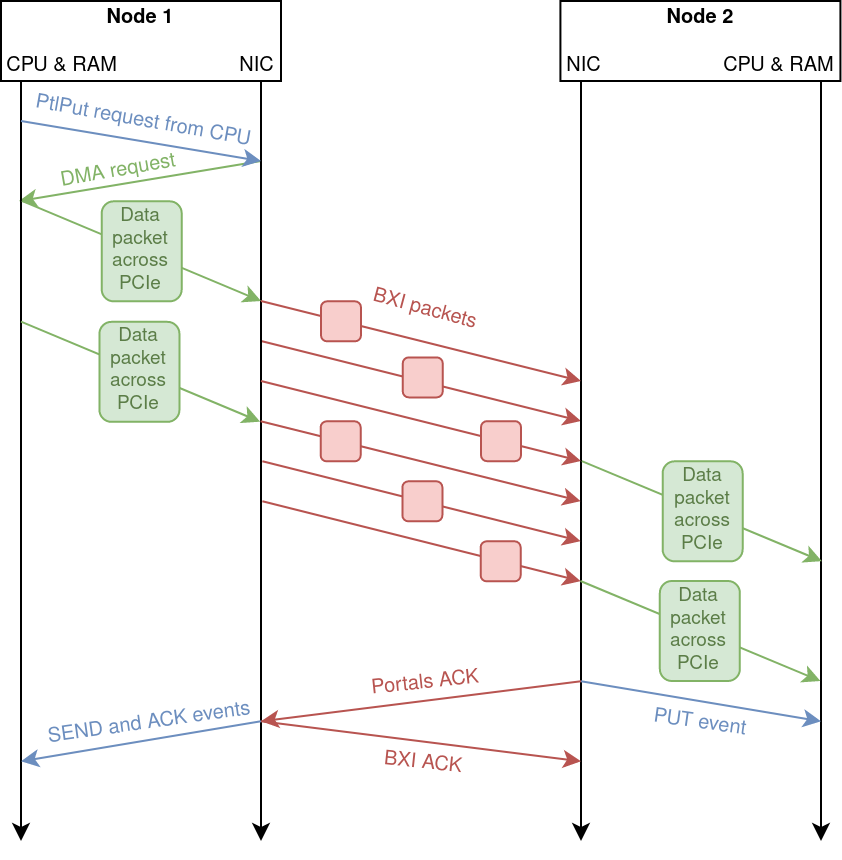
\includegraphics[width=0.9\textwidth]{4_portals/PCI_transfer_real.png}
    \caption{Data transfers when performing a DMA on real hardware}
    \label{fig:4_portals:PCI_transfer_real}
\end{figure}

For the biggest messages, DMA (Direct Memory Access) is used: the CPU simply
sends a command containing the address and length of the memory to be
transferred, and then the NIC reads the memory when it processes the command.
Since the Portals library is mostly operating in userland (and not from a kernel
driver), this means that the addresses sent to the NIC are virtual. This is why
the NIC features a Virtual To Physical (V2P) component which implements the same
page walk through the Memory Management Unit (MMU) as the CPU does, in order to
request the physical memory address and send the data on the network.
Additionally, it is important to note that during a communication using DMA,
three transfers happen in total: a data read across PCI at the sender, the
network transfer, and a data write across PCI at the receiver. Both the sender
and the receiver of the payload synchronize on all three data transfers, which
are dependent on each other: these transfers are all made of packets, and at the
lowest level, flow control guarantees that the data progresses at a rhythm that
is sustainable by both NICs using a flit-level credit system. This means that,
as depicted in Figure~\ref{fig:4_portals:PCI_transfer_real}, PCI packets (which
are typically 512B, even though 256 and 1024B are also supported by BXI) are
broken down into 32B flits, which are then packed into 72B BXI link-level
packets (which contain two flits and 8B of header metadata), and then
re-assembled into PCI packets to be written at the target side.

On the other hand, when sending data back in a response at target side (after a
\inline{PtlGet} for example), the data transfer from memory to the NIC is
always performed in the DMA style, since the targeted machine does not know
which piece of memory might be requested and when.

\subsubsection{Model in S4BXI}

In S4BXI, the inline and PIO transfers are modeled exactly as they happen in the
BXI NIC (with easy to configure thresholds which allow testing different
hypothetical scenarios). The DMA transfers, on the other hand, are by essence
difficult to model because of the nature of our flow model. Indeed, as presented
previously, in the event of a DMA we have three different transfers that are all
dependent on each other, and this dependency can only be described accurately by
modeling each packet. This section will present several ways to model these
transfers, starting with the most naive and ending with the model that is
currently implemented in our simulator.

\begin{figure}[!ht]
    \centering
    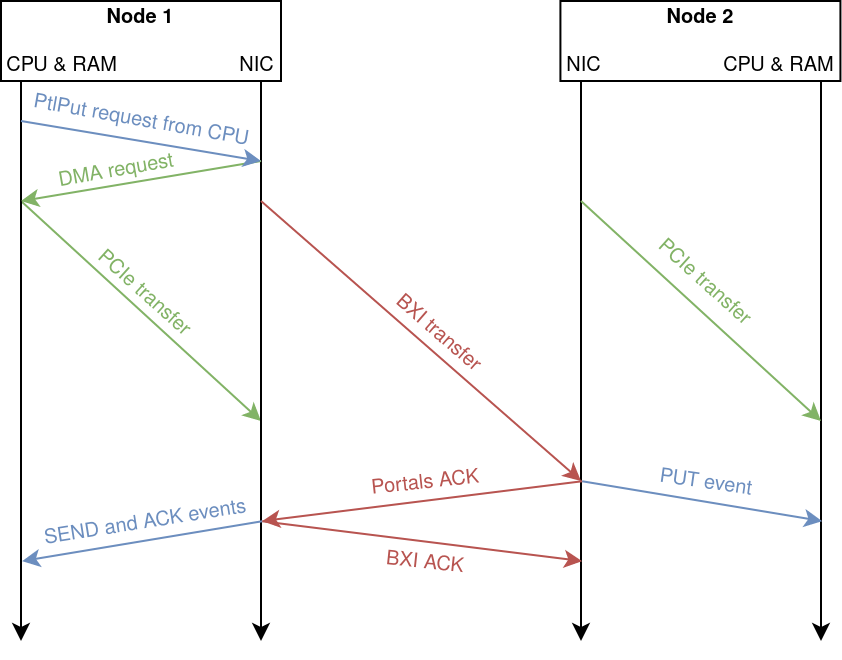
\includegraphics[width=0.9\textwidth]{4_portals/PCI_transfer_naive.png}
    \caption{Naive flow model of data transfers when performing a DMA}
    \label{fig:4_portals:PCI_transfer_naive}
\end{figure}

A naive way to model this would be to start all three transfers at the same time
in simulation (since they are very well pipelined in real life), as depicted in
Figure~\ref{fig:4_portals:PCI_transfer_naive}. While this is a good
approximation for moderate workloads, it loses significant accuracy if there is
congestion on any of the transfers. In particular, the PCI write at the receiver
will progress even if the BXI transfer gets slowed down by congestion. This
results in an overly optimistic simulator in the case of communication-intensive
workloads.

\begin{figure}[!ht]
    \centering
    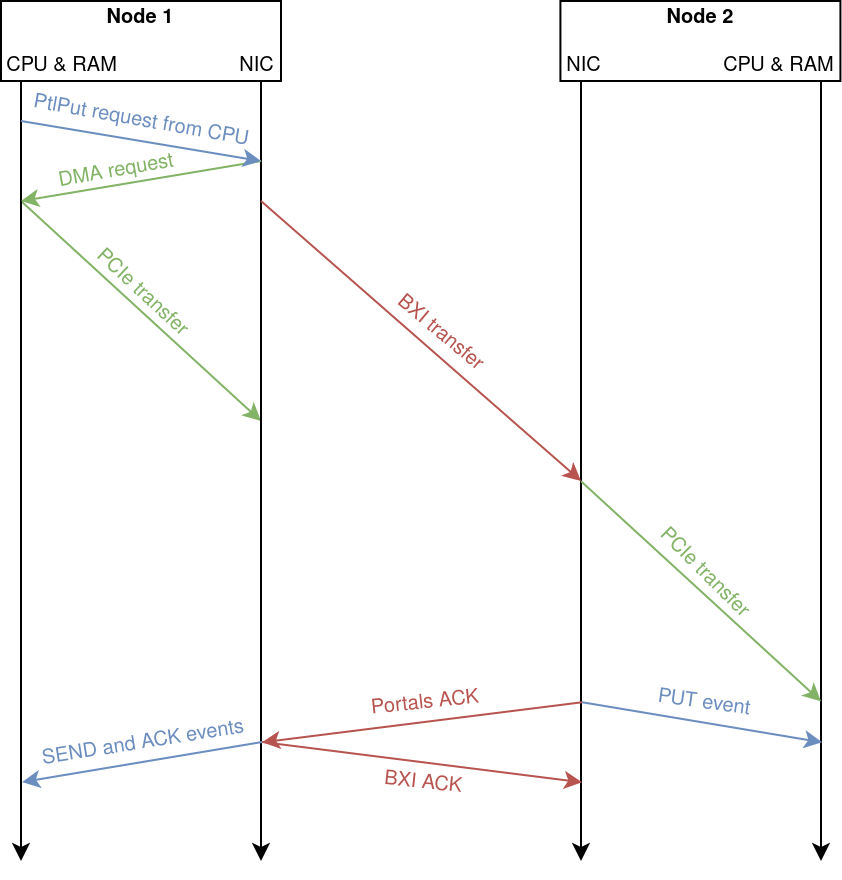
\includegraphics[width=0.9\textwidth]{4_portals/PCI_transfer_late_events.png}
    \caption{Flow model of data transfers when performing a DMA, accounting for network congestion}
    \label{fig:4_portals:PCI_transfer_late_events}
\end{figure}

A different option to model this scenario is to perform the PCI write at target
only when the network transfer across BXI is complete, as depicted in
Figure~\ref{fig:4_portals:PCI_transfer_late_events}. While this model accounts
for congestion across the BXI network, it is very pessimistic in most cases,
effectively reducing the maximum achievable bandwidth to half the bandwidth of
the BXI cables, since the BXI transfer and the PCI write are performed sequentially.

\begin{figure}[!ht]
    \centering
    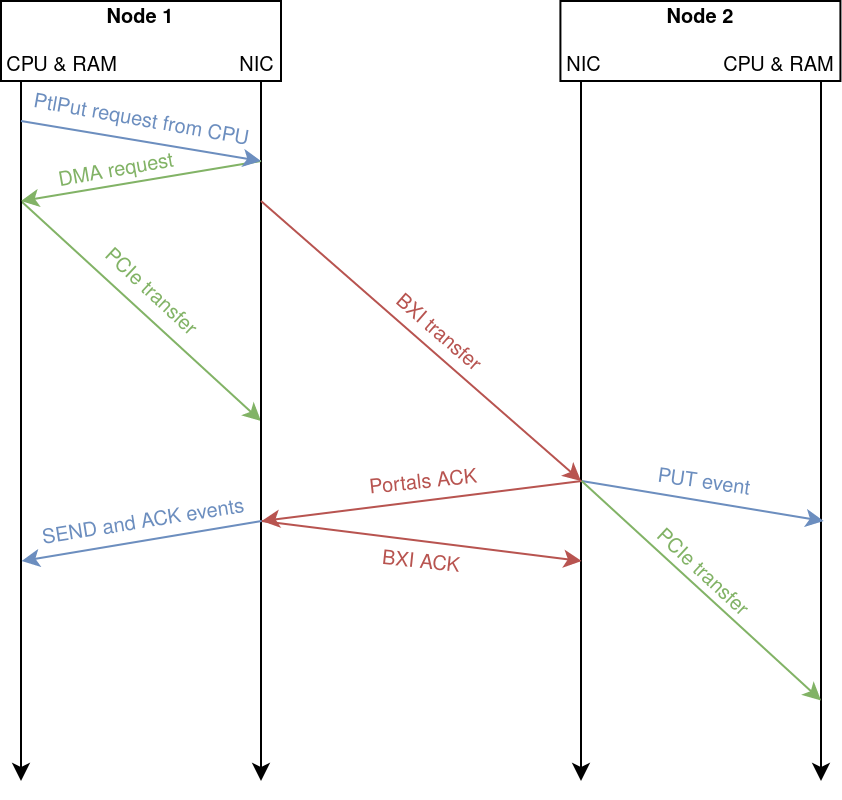
\includegraphics[width=0.9\textwidth]{4_portals/PCI_transfer_early_events.png}
    \caption{Flow model of data transfers when performing a DMA, with asynchronous PCI writes}
    \label{fig:4_portals:PCI_transfer_early_events}
\end{figure}

Finally, a solution to delay the PCI write while generating Portals events and
acknowledgements faster is to perform the PCI write asynchronously in the
background, as depicted in Figure~\ref{fig:4_portals:PCI_transfer_early_events}.
While this is still very far from a perfect model, it will generate a more
realistic congestion on the PCI bus at receiver side, which will impact the
generation of PUT events for example.

It is important to note that in any case, all these models are only realistic
for large data transfers, in which the payload is composed of many PCI packets.
Indeed, we can see on Figure~\ref{fig:4_portals:PCI_transfer_real} that even
though the three types of transfers are very well pipelined, the first PCI
packet at sender side needs to be fully received before initiating the transfer
across BXI, and at receiver side, the BXI transfer needs to be fully completed
before starting to write the last PCI packet. This means that for messages which
can fit in a few PCI packets, the pipeline will not allow the transfers to
overlap perfectly. The most pathologic case would be for messages that fit in a
single PCI packet (so smaller than 512B), for which there is no pipelining at
all, and the three transfers are essentially sequential. In S4BXI we account for
this effect by adding a small sleep inside TX Actors before starting the
transfer across BXI, and another similar sleep in RX Actors before generating
Portals events and any acknowledgement. Therefore, the final sequence of
transfers that is implemented in S4BXI corresponds to
Figure~\ref{fig:4_portals:PCI_transfer_simu_final}.

\begin{figure}[!ht]
    \centering
    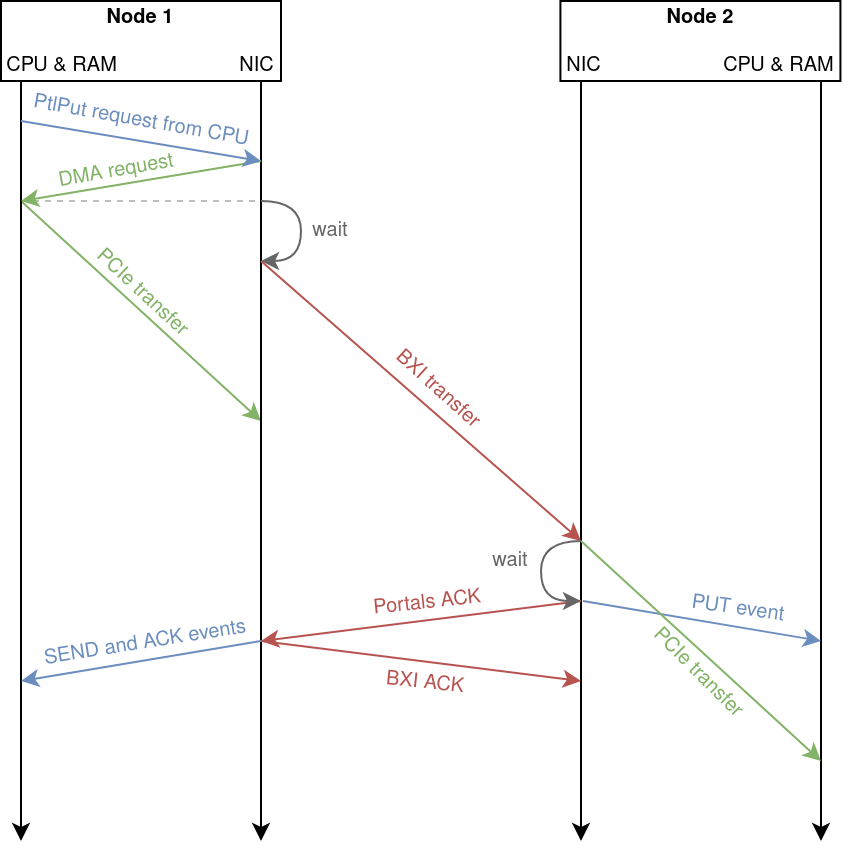
\includegraphics[width=0.9\textwidth]{4_portals/PCI_transfer_simu_final.png}
    \caption{Flow model of data transfers when performing a DMA, as implemented in S4BXI}
    \label{fig:4_portals:PCI_transfer_simu_final}
\end{figure}

Finally, it is also important to mention that all transfers that are represented
in each figure only model the time that operations take in our simulator: since
our simulation is single-threaded, the data that is exchanged between two NICs
is available at the target instantly by exchanging a C pointer. Therefore, it is
not erroneous to issue a PUT event before the end of the PCI write at target
side, as the RX side of our simulated NIC can access the payload at any point.

\subsection{Performance options}

In a first attempt to customize the performance/accuracy tradeoff of the
simulator, we have implemented several options that can simplify the processing
inside our simulated NICs:

\subsubsection{Quick ACKs}

Very often, messages containing data (\inline{PtlPut} requests for example) are
much heavier than lightweight acknowledgements, and will account for the
majority of the time spent performing network operations on a real-world
cluster. Therefore, S4BXI allows generating ACK events instantaneously instead
of creating a proper ACK message and sending it on the network. This means that
in this case, ACK events at sender side are going to be generated from an RX
Actor at the \textbf{receiver} side, which is obviously possible in simulation
only (since it would require a network communication in the real world). If E2E
processing is active, enabling this option saves not only one but two small ACK
messages: the Portals ACK used to generate the ACK event, and the BXI ACK used
by E2E internally, as depicted in Figure~\ref{fig:4_portals:quick_acks}

\begin{figure}[!ht]
    \centering
    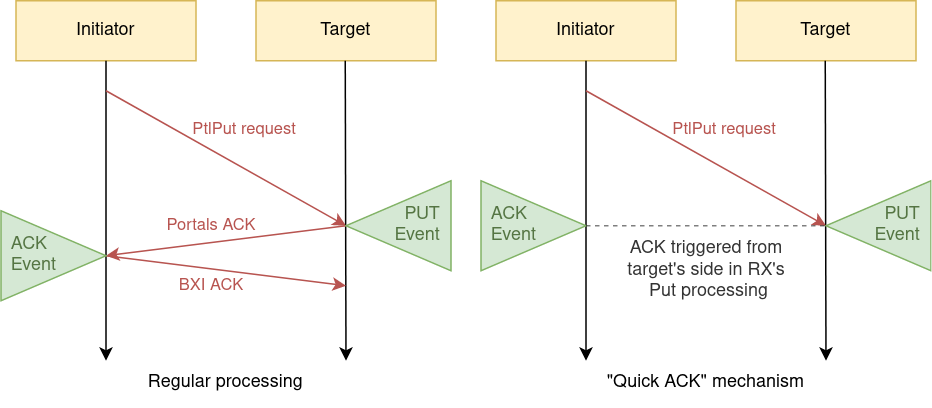
\includegraphics[width=1\textwidth]{4_portals/quick_acks.png}
    \caption{Quick ACK mechanism in S4BXI}
    \label{fig:4_portals:quick_acks}
\end{figure}

\subsubsection{Simplified PCI model}

In the same spirit as Quick ACKs, S4BXI supports ignoring small PCI transfers:
if messages of a consequent size are exchanged on the network, the time spent
exchanging lightweight commands across the PCI bus in real world is usually
negligible compared to data transfers (writes at target side or reads at
initiator side). Therefore, S4BXI provides an option to ignore them and save a
few operations in SimGrid's kernel, which is controlled either globally using
the \inline{S4BXI_MODEL_PCI_COMMANDS} environment variable, or on an Actor per
Actor basis using the \inline{model_pci_commands} property in the simulation's
deployment. A more aggressive optimization consists in disabling every PCI
transfer (including data transfers) completely. While this can increase
performance a bit more, it is much less realistic. Similarly, this option can be
enabled globally using the \inline{S4BXI_MODEL_PCI} environment variable, or
locally using the \inline{model_pci} property on individual Actors.

\section{Tracing and Visualization System}

While SimGrid provides a low-level tracing system, which allows logging all
activity on compute resources, links, etc., we felt the need to create our own
too. Since it operates at Portals level, our system can add more metadata to
operations: this provides a precise log of the different request and response
types, whereas SimGrid's low-level system only provides the usage of each Link,
without any information on the type of Portals operation.

Tracing in S4BXI is disabled by default. To enable it, one simply sets the
environment variable \inline{S4BXI_LOG_FOLDER} to a valid path. S4BXI will
then write logs of all operation in CSV format (for easier parsing), splitting
the log file every 10,000 lines. Additionally, the variable
\inline{S4BXI_LOG_COMPUTATION} controls whether CPU operations should be
logged, or only network ones (since CPU operations can be very numerous, and not
necessarily the main point of interest).

\begin{figure}[!ht]
    \lstinputlisting[basicstyle=\ttfamily\footnotesize,frame=bt,language=C++]{4_portals/bxi_log_type.cpp}
    \caption{Event types in S4BXI's tracing system}
    \label{fig:4_portals:bxi_log_type}
\end{figure}

\begin{figure}[!ht]
    \centering
    \includegraphicsOverflow{4_portals/S4BXI_trace.png}{1.15}
    \caption{Example trace from S4BXI, two simple Put requests between NID 1 and 2}
    \label{fig:4_portals:S4BXI_trace}
\end{figure}

The different types of events logged by S4BXI is described in the enum
\inline{bxi_log_type}, which is shown in
Figure~\ref{fig:4_portals:bxi_log_type}. The output CSV files can be easily
parsed, but to simplify their visualization we developed a small online
tool\footnote{Hosted at \url{https://s4bxi.julien-emmanuel.com/log-viewer/}} to
display operations in a sequence graph. While it does not scale very well when
the number of nodes involved is important, it is a useful tool to debug at a
small scale, and its code\footnote{Open source at
\url{https://framagit.org/s4bxi/s4bxi-log-viewer}} gives a simple example of how
to use the trace files. A screenshot of an example output of our tool is
displayed on Figure~\ref{fig:4_portals:S4BXI_trace}.

\section{Additional implementation considerations}

\subsection{Practical usage of S4BXI, and simulated process isolation}
\label{subsec:4_portals:process_isolation}

\begin{figure}[!ht]
    \centering
    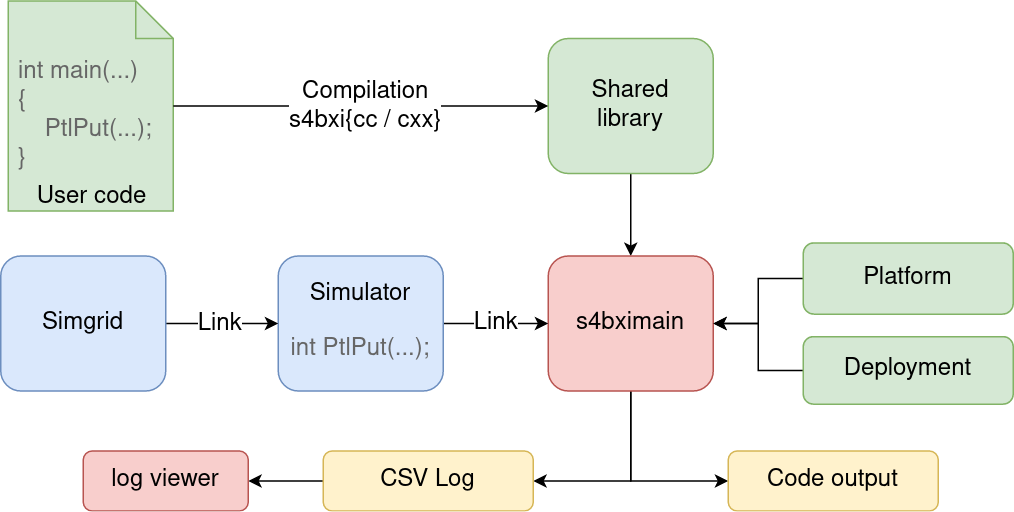
\includegraphics[width=0.9\textwidth]{4_portals/s4bxi_usage.png}
    \caption{S4BXI components and usage}
    \label{fig:4_portals:s4bxi_usage}
\end{figure}

To facilitate the configuration of the compiler for S4BXI users we provide
scripts that act as wrappers around compilers (namely \inline{s4bxicc} and
\inline{s4bxicxx}) that have a very similar goal than the corresponding
\inline{smpicc} and \inline{smpicxx}: make the compiled program a shared
library, and include header files to redefine the symbols that we want to
capture (using C macros). An overview of the methodology is shown on
Figure~\ref{fig:4_portals:s4bxi_usage}: First the application's code is
compiled, either with our compiler wrappers directly or simply by adding the
\inline{-shared} flag manually. Then S4BXI is started (through the binary
\inline{s4bximain}) with three essential arguments: the simulated platform's
description, the associated deployment configuration, and finally the shared
library which contains the application. Each Actor which runs the user
application will then copy the application's library on disk with a different
name for each simulated process, and use the \inline{dlopen} and \inline{dlsym}
function to extract the \inline{main} symbol from the library and run it. The
reason for copying the simulated application (instead of opening the same
library from every simulated process) is that it allows us to trick the dynamic
linker into thinking that all these copies are different libraries, which allows
us to leverage the linker's ability to isolate the global symbols (in particular
global variables) of different libraries running in the same address space. This
provides isolation between the different simulated processes even though they
all run in a single thread in practice, without having to implement this feature
ourselves.

\subsection{Platform implementation in S4BXI}

At the beginning of this PhD, the most popular way of describing SimGrid
platforms was using a static XML document\footnote{The corresponding DTD is
available at \url{https://simgrid.org/simgrid.dtd}}. Unfortunately, this wasn't
a very flexible approach: there are XML tags that try to simplify the platform,
such as \inline{<cluster>} which creates the complete list of Hosts and Links
for common topologies, but unfortunately when using these the ``leaf'' nodes of
the cluster could only be simple Hosts (instead of the more complete model with
PCI cables, etc. that we described above). For this reason we made some scripts
to convert the output of real-world cluster management software (BXI-AFM in our
case) into a SimGrid XML platform that comply with S4BXI's requirements. While
this is a functional solution, it had the downside of generating potentially
very heavy and verbose platforms, which could take a significant amount of time
and memory to parse in SimGrid. Thankfully, since then the SimGrid team
developed a C++ API (integrated in S4U) to describe platforms, which is
significantly more performant and flexible. We added support for it in our
simulator by checking the filetype of the platform at startup (either an XML
file or a shared library compiled from a C++ platform), and in the case of a C++
platform our simulator looks for a specific symbol (\inline{load_platform}) to
call, which is responsible for generating the platform. While we kept the
support for XML platforms, all our experiments will use the C++ API, which
should become the standard way of using SimGrid in the future.

\subsection{Portals's implementation in C/C++}

\begin{figure}[!ht]
    \centering
    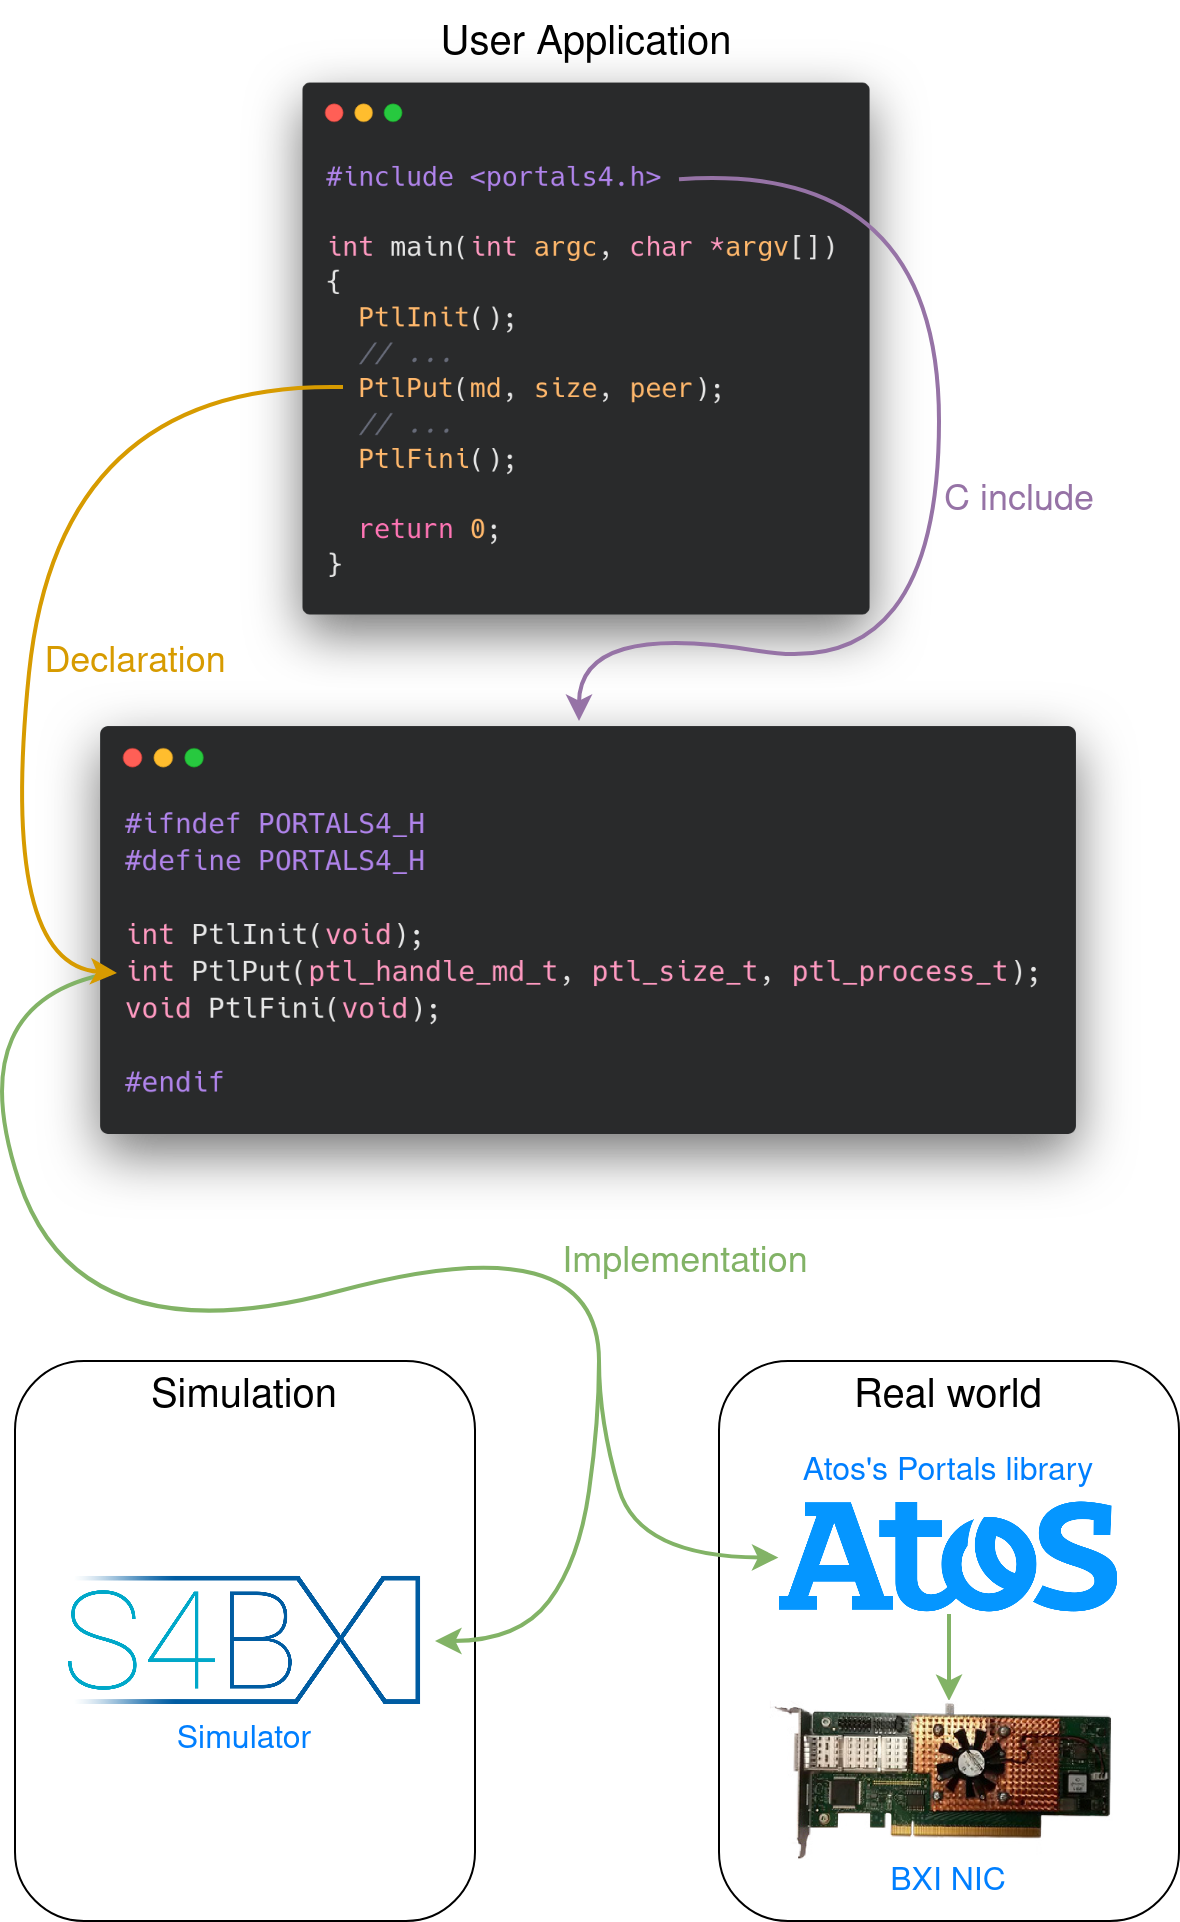
\includegraphics[width=0.7\textwidth]{4_portals/portals_h.png}
    \caption{Declaration and implementation of Portals's primitives}
    \label{fig:4_portals:portals_h}
\end{figure}

On a real cluster, the user code (or a library such as MPI) includes the
\inline{portals4.h} header file, which provides the declarations for Portals's
structures and primitives. In simulation, we simply reuse the
\inline{portals4.h} header provided by the real world implementation made by
Atos (as well as a few BXI-specific helpers for an optimal compatibility,
\inline{portals4_bxiext.h} and \inline{portals4_services.h}). These files allow
us to have identical declarations, so that user code can use our simulated
Portals or Atos's one transparently. The difference comes from the
implementation: while the Portals primitives are implemented by Atos's library
on a real cluster, in simulation S4BXI provides an implementation on top of
SimGrid. This methodology is represented on
Figure~\ref{fig:4_portals:portals_h}, in which we can see how the difference
between real-world and simulation comes only from the implementation of
primitives.

Internally all our Actors are implemented by C++ classes, as SimGrid is very
flexible in this regard: Actors' behavior can be implemented either using a
simple function, a class, or anything that is callable (our complete class
hierarchy is represented in Appendix~\ref{app:s4bxi_class_hierarchy}. Therefore,
the implementation behind the public interface is simply a small layer that
retrieves the current S4BXI Actor instance (\inline{BxiMainActor} in our class
hierarchy) and calls a member function corresponding to the desired Portals
primitive. This lookup of the current S4BXI Actor instance is optimized using a
small plugin we wrote for SimGrid, which allows us to store this pointer in
SimGrid's representation of Actors.

\subsection{Capturing function calls}

While the Portals primitives naturally link with S4BXI's implementation in
simulation, there are other function calls that need to be
intercepted: all utilities that rely on time, such as
\inline{gettimeofday}, \inline{sleep}, etc. must be
re-implemented in simulation in order to use simulated time instead of
wall-clock time. A traditional way to perform this interception is to preload a
library using the \inline{LD_PRELOAD} environment variable on Linux. While
this is efficient, we chose a simpler approach (similar to SMPI) where the
function calls that we re-implent are redirected to the simulator's
implementation using \inline{#define} C macros. This method is more intrusive
since it requires re-compiling the simulated application, but in our workflow it
does not add any constraint since we already need to compile the application, in
order to make a shared library (as explained in
Subsection~\ref{subsec:4_portals:UserAppActors}).

In S4BXI we implemented most functions that can be used to sleep with various
precision (\inline{sleep}, \inline{nanosleep}, etc.), functions to query the
current time (\inline{gettimeofday}, \inline{clock_gettime}, etc.) as well as a
few other utilities such as \inline{hostname}, \inline{getpid}, etc. so that
each simulated node returns a value from the simulated world instead of data
from the machine running the simulation. We also support a subset of signal
handlers that we encountered in low-level benchmarks: \inline{sigaction} stores
the handler for a given signal in a simulated-Actor specific structure, and this
handler is then executed after a call to \inline{setitimer} or \inline{alarm}
and the corresponding waiting time is elapsed in the simulated world. In order
to wait for the desired amount of time, and call the appropriate handler when
the timeout expires, we spawn a short-lived Actor so that the main application
can continue to progress at the same time, as it would in real-life (since the
timer runs in the background).

\subsection{Completeness}

S4BXI was made with the end goal of simulating high-level APIs, in particular
MPI, and therefore we only implemented the features that we needed for this
purpose. This means that our Portals implementation is not complete, although
the majority of Portals primitives are supported (and tested in our Continuous
Integration). The main missing features are I/O Vectors (IOVEC), which are the
ability to send several pieces of non-contiguous data at once, as well as
triggered operations, which are the ability to send a message automatically when
a specific event happens in Portals. We only left these features aside because
of time constraints, and we believe that the current architecture of our
simulator would make their implementation straightforward. Adding these features
would only be a matter of investing some engineering time, if there was a need
for it, since they would be very similar to the existing logic currently
implemented in the simulator.

\section{Experimental validation}
\label{sec:4_portals:validation}

In order to get a first validation of our Portals model (before moving on to
higher-level APIs) we executed two types of benchmark on a BXI cluster and in
S4BXI: first we started with custom-made tests, which are very simplistic, and
then we ran PtlPerf, which is a pre-existing tool made at Atos to perform
point-to-point performance measurements, as presented in
Section~\ref{sec:2_context_hpc:benchmarks}.

\subsection{Custom made benchmarks}

While we check that all request types are functionnally correct in our
Continuous Integration, we studied in more detail \inline{PtlPut} and
\inline{PtlGet} operations in order to validate their performance in simulated
time against real-world executions on BXI hardware. Indeed, it is easy to write
a test suite to ensure that all operations transfer data correctly, but
evaluating the accuracy of the simulator is significantly harder to automate. We
chose to study these primitives because they are the most commonly used, in
particular they are the only request types that are used in the MPI
implementation that we will study in the next chapter.

\subsubsection{Benchmarks' behavior}

Each benchmark that we made operates on the same principle: 10,000 requests (Put
or Get) are sent from a machine A to a machine B, while both machines measure
the total time. This workload is repeated for 64 different message sizes,
which are chosen according to the following method: the first few message sizes
are hardcoded and correspond to the sizes where we expect significant changes in
the duration of the benchmark (because of the optimizations that we know exist
in the real-world hardware and the S4BXI model), for example at 64B (and
therefore 65B too in order to see the change clearly). Then, the next sizes are
generated at random, using a distribution uniform on a log scale (in base two).
We did not go for powers of two directly, to avoid testing only very particular
values. We also did not go for a simple uniform distribution because we are more
interested in small values, for which there are more variations in the
performance of BXI.

We designed five types of benchmarks: three for the \inline{PtlPut} operation
and two for \inline{PtlGet}. To make this section easier to read, we will name
each of these variants, and illustrate them with sequence diagrams (which offer
a simplified representation of the transfers involved, in particular they are a
lot less detailed than figures~\ref{fig:4_portals:PCI_transfer_naive}
to~\ref{fig:4_portals:PCI_transfer_simu_final}):

\begin{description}
    \item[Put-WaitAck] performs Put operations. The benchmark waits for an ACK
    event before moving on to the next operation, which means that there is only
    one message inflight at all times. This corresponds to the sequence diagram
    on Figure~\ref{fig:4_portals:ptlput_waitack_seq}.
    \item[Get-WaitReply] performs Get operations. The benchmark waits for a
    REPLY event before moving on to the next operation, so once again there is
    only one message inflight at all times. This corresponds to the sequence
    diagram on Figure~\ref{fig:4_portals:ptlget_waitreply_seq}.
    \item[Put-NoWait] performs Put operations as fast as possible, without
    waiting for any event. While this workload is not a very realistic use of
    BXI NICs, it allows us to benchmark the ability of the NIC to absorb and
    process many commands, and to see how the network performs when many
    messages are inflight at the same time. This corresponds to the sequence
    diagram on Figure~\ref{fig:4_portals:ptlput_nowait_seq}.
    \item[Get-NoWait] performs Get operations as fast as possible, without
    waiting for any event. Once again this benchmark allows us to stress the
    NICs involved, in particular the target NIC which will receive many requests
    at a high rate. This corresponds to the sequence diagram on
    Figure~\ref{fig:4_portals:ptlget_nowait_seq}.
    \item[Put-WaitSend] performs Put operations. The benchmark waits for a SEND
    event before moving on to the next operation. This is closer to a realistic
    use case of Portals, as this event indicates that the source buffer can be
    safely reused. In practice, it allows small messages to be processed in a
    pipelined way, while for large messages it is equivalent to waiting for the
    ACK event. This corresponds to the sequence diagram on
    Figure~\ref{fig:4_portals:ptlput_waitsend_seq}.
\end{description}

\begin{figure}[!h]
    \centering
    \begin{subfigure}{.5\textwidth}
        \centering
        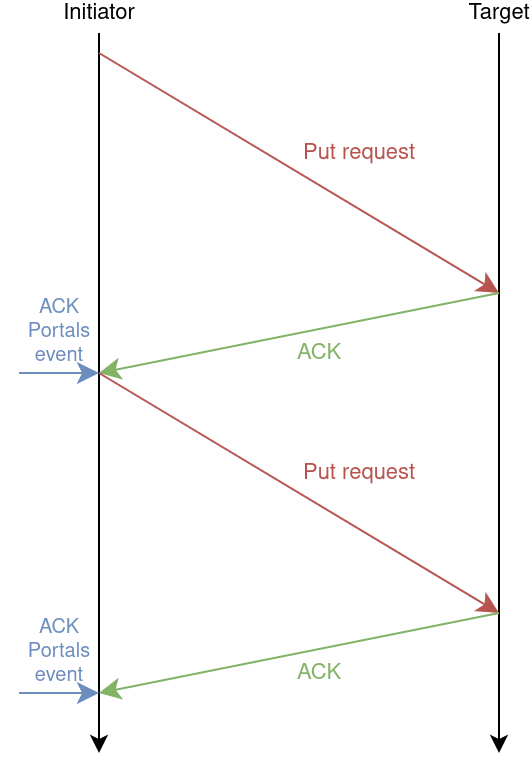
\includegraphics[width=1\linewidth]{4_portals/bench_put_waitack.png}
        \caption{\inline{PtlPut} variant (\textbf{Put-WaitAck})}
        \label{fig:4_portals:ptlput_waitack_seq}
    \end{subfigure}% this comment is important otherwise the images are vertical
    \begin{subfigure}{.5\textwidth}
        \centering
        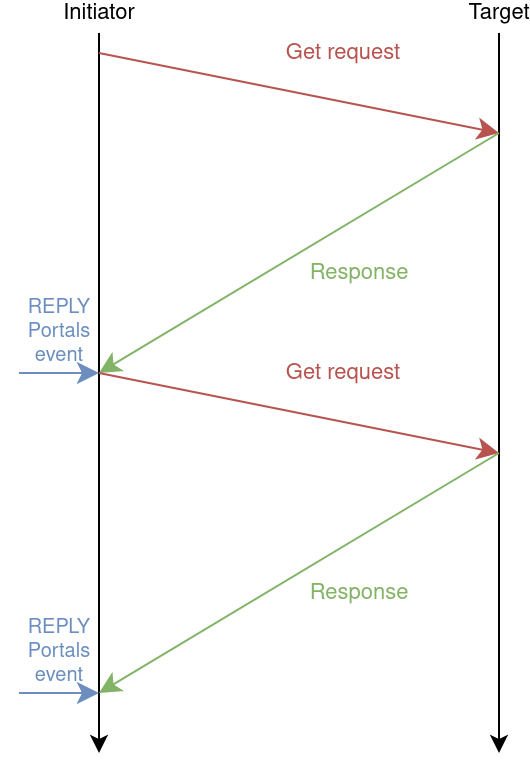
\includegraphics[width=1\linewidth]{4_portals/bench_get_waitreply.png}
        \caption{\inline{PtlGet} variant (\textbf{Get-WaitReply})}
        \label{fig:4_portals:ptlget_waitreply_seq}
    \end{subfigure}
    \caption{Portals experiment, one request at a time}
    \label{fig:4_portals:ptl_wait_seq}
\end{figure}

\begin{figure}[!h]
    \centering
    \begin{subfigure}{.5\textwidth}
        \centering
        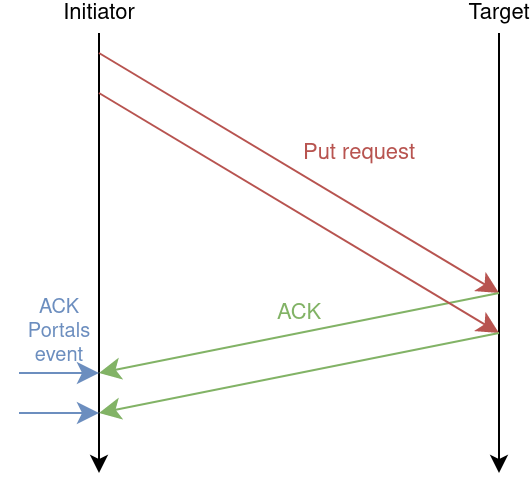
\includegraphics[width=1\linewidth]{4_portals/bench_put_nowait.png}
        \caption{\inline{PtlPut} variant (\textbf{Put-NoWait})}
        \label{fig:4_portals:ptlput_nowait_seq}
    \end{subfigure}% LaTeX is garbage
    \begin{subfigure}{.5\textwidth}
        \centering
        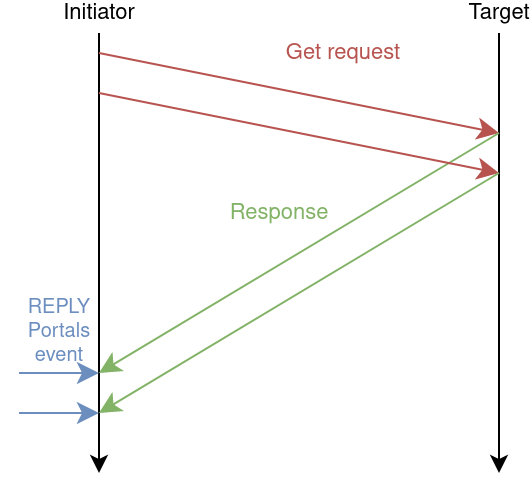
\includegraphics[width=1\linewidth]{4_portals/bench_get_nowait.png}
        \caption{\inline{PtlGet} variant (\textbf{Get-NoWait})}
        \label{fig:4_portals:ptlget_nowait_seq}
    \end{subfigure}
    \caption{Portals experiment, sending requests as fast as possible}
    \label{fig:4_portals:ptl_nowait_seq}
\end{figure}

\begin{figure}[!h]
    \centering
    \begin{subfigure}{.5\textwidth}
        \centering
        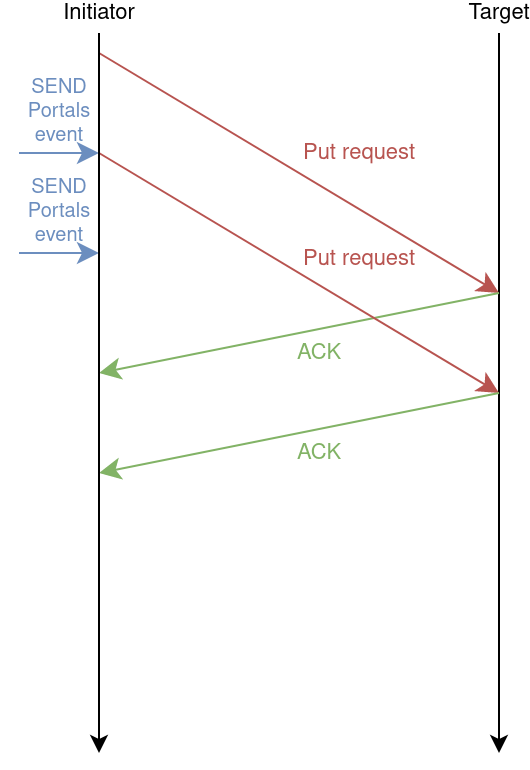
\includegraphics[width=1\linewidth]{4_portals/bench_put_waitsend_small.png}
        \caption{Messages smaller than 64B}
        \label{fig:4_portals:ptlput_waitsend_small_seq}
    \end{subfigure}% LaTeX is garbage
    \begin{subfigure}{.5\textwidth}
        \centering
        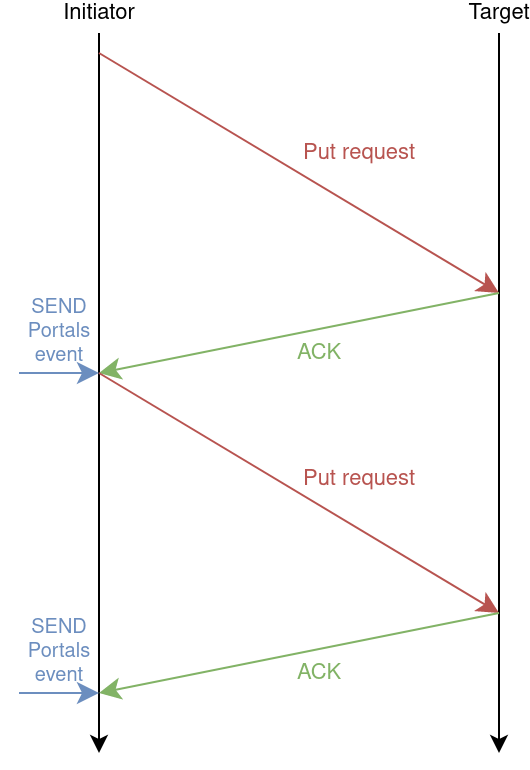
\includegraphics[width=1\linewidth]{4_portals/bench_put_waitsend_big.png}
        \caption{Messages bigger than 64B}
        \label{fig:4_portals:ptlput_waitsend_big_seq}
    \end{subfigure}
    \caption{\inline{PtlPut} experiment, waiting for SEND event between requests (\textbf{Put-WaitSend})}
    \label{fig:4_portals:ptlput_waitsend_seq}
\end{figure}

As illustrated on figure~\ref{fig:4_portals:ptl_wait_seq}, the
\textbf{Put-WaitAck} and \textbf{Get-WaitReply} benchmarks are very simplistic,
as they evaluate the total latency of an operation, which includes an initial
message and a response (either a full reply or a small ACK). On the other hand,
Figure~\ref{fig:4_portals:ptl_nowait_seq} shows that the \textbf{Put-NoWait} and
\textbf{Get-NoWait} benchmarks stress both NICs involved much more, by
requesting as many operations inflight as possible, which evaluates the capacity
of the hardware to process commands and incoming messages in a pipelined way.
Finally, \textbf{Put-WaitSend} corresponds to a more realistic usage of the
hardware.

\subsubsection{Experimental setup}

When simulating these benchmarks, we observed that our simplistic CPU model
caused the simulations to be overly pessimistic (to the point where putting a
zero nanosecond latency on all Links of our simulated platform still gave
pessimistic results). We concluded that since our benchmarks are focused on the
network, the CPU sections between two network primitives are very short, and
that the latency of starting and stopping our CPU timer impacted its
measurements in a very significant way, resulting in pessimistic CPU times. To
fix this problem, we can configure the CPU model to ignore computations that are
shorter than a supplied threshold, therefore for these experiments we ignored
all computations smaller than one microsecond, which effectively ignores all
computation phases in this specific case (since the CPU time is only spent
executing a \inline{for} loop around the network primitives essentially).

From a technical point of view, in the real-world cluster the nodes we use are
equipped with BXI v2 hardware and AMD EPYC™ 7763 64-Core processors. For the
simulations we use a traditional desktop computer, which has an Intel® Core™
i9-10850K CPU and 32 GB of RAM. For each message size the experiment is executed
five times on the real-world cluster in order to ensure that the results are
consistent, and only once in simulation since it is fully deterministic and
reproducible.

\subsubsection{Results}

The results of our benchmarks are displayed on the following figures:
\begin{itemize}
    \item Figure~\ref{fig:4_portals:ptlput_waitack} shows the result of the
    \textbf{Put-WaitAck} benchmark
    \item Figure~\ref{fig:4_portals:ptlput_nowait} shows the result of the
    \textbf{Put-NoWait} benchmark
    \item Figure~\ref{fig:4_portals:ptlput_waitsend} shows the result of the
    \textbf{Put-WaitSend} benchmark
    \item Figure~\ref{fig:4_portals:ptlget_waitreply} shows the result of the
    \textbf{Get-WaitReply} benchmark
    \item Figure~\ref{fig:4_portals:ptlget_nowait} shows the result of the
    \textbf{Get-NoWait} benchmark
\end{itemize}

\begin{figure}[!h]
    \centering
    \includegraphicsOverflow{4_portals/custom/put_waitack.png}{1.2}
    \caption{\textbf{Put-WaitAck} benchmark}
    \label{fig:4_portals:ptlput_waitack}
\end{figure}

\begin{figure}[!b]
    \centering
    \includegraphicsOverflow{4_portals/custom/put_nowait.png}{1.2}
    \caption{\textbf{Put-NoWait} benchmark}
    \label{fig:4_portals:ptlput_nowait}
\end{figure}

\begin{figure}[!b]
    \centering
    \includegraphicsOverflow{4_portals/custom/put_waitsend.png}{1.2}
    \caption{\textbf{Put-WaitSend} benchmark}
    \label{fig:4_portals:ptlput_waitsend}
\end{figure}

\begin{figure}[!b]
    \centering
    \includegraphicsOverflow{4_portals/custom/get_waitreply.png}{1.2}
    \caption{\textbf{Get-WaitReply} benchmark}
    \label{fig:4_portals:ptlget_waitreply}
\end{figure}

\begin{figure}[!h]
    \centering
    \includegraphicsOverflow{4_portals/custom/get_nowait.png}{1.2}
    \caption{\textbf{Get-NoWait} benchmark}
    \label{fig:4_portals:ptlget_nowait}
\end{figure}

Each graph shows the overall duration of the benchmark, the bandwidth, and the
message rate, estimated by our simulator in red (with circular points) and as
reported by real-world runs on the BXI cluster in blue (with triangular points).
It is important to note that all graphs use a log scale on both axes (a base two
log on the x-axis and a base ten log on the y-axis), in order to make results
more readable. In particular, on all variants of our experiments, the left side
shows experiments on small messages, therefore the duration of operations
correspond to the latency of the hardware, whereas on the right side the
duration of operations is dominated by the bandwidth of network cables. This
explains why for large messages, all benchmarks exhibit the same behavior (which
is perfectly captured by our simulator, as it is the easiest workload to model).

While most results given by our simulator are very good, there are a few notable
things to see in these graphs: first, the benchmarks that perform one request at
a time give excellent results in simulation. This is because these benchmarks
mainly evaluate the latency of the network, which we can tune easily, without
caring about the ability of the NIC to process requests in parallel (or at least
in a pipelined way). On the other hand, benchmarks which send requests as fast
as possible give results which are further from reality: it is harder to model
these cases because the performance of the benchmark depends on the ability of
the NIC to process requests quickly, and not only on the latency of the network.
This is particularly difficult to estimate because of the tradeoff that we
chose: since we use a flow model, and not a cycle accurate emulator of the NIC,
the blocking time that the NIC needs to process requests can only be accounted
for using approximate heuristics involving small \inline{sleep()}s of a few
hundred nanoseconds in the Actors of the NIC. This is a known limitation of this
type of model, and we carefully tuned these delays, which shows very good
results for \inline{PtlPut} operations
(Figure~\ref{fig:4_portals:ptlput_nowait}), and acceptable results for
\inline{PtlGet} requests (Figure~\ref{fig:4_portals:ptlget_nowait}).

For \inline{PtlPut} operations specifically, we can see that the graphs are very
similar whether we wait for the full completion of requests
(Figure~\ref{fig:4_portals:ptlput_waitack}), or just the SEND events
(Figure~\ref{fig:4_portals:ptlput_waitsend}). This is expected since for
messages larger than 64B the SEND event is issued at the very end of the
request's life. For small messages on the other hand, we can see that only
waiting for the SEND event allows several requests to be processed in a
pipelined way, resulting in lower latencies which are correctly modeled by
S4BXI. Overall, the results of our simulators are excellent for these types of
benchmarks, as they perfectly capture all the changes in performance that can be
seen on the real-world experiment. This accuracy of S4BXI comes directly from
our low-level model of the hardware, and in particular our model of PCI
transfers, since different message sizes allow NICs to perform different
optimizations on these transfers, which we were able to capture in S4BXI
(without having to use packet-level simulation).

For \inline{PtlGet} operations, we can see that when sending them one at a time
(Figure~\ref{fig:4_portals:ptlget_waitreply}), there is a small performance gap
around 64B. On one hand this is not very surprising, since we have already
established that 64B is a specific value for BXI NICs, which is a usual
threshold to be able to apply some optimizations (or not). The problem in this
case is that for Get requests, there should not be any particular optimization
of this sort as far as we are aware, which was confirmed by the hardware
designers of the NIC (who were kind enough to answer all our questions to the
best of their ability). Therefore, we did not model this performance gap in
S4BXI, since its origin in the real world is unknown. While this is not the most
satisfying conclusion, the performance gap is small enough that we do not expect
it to cause a significant accuracy loss in the rest of our work, especially
since the \inline{PtlPut} primitive is more commonly used than \inline{PtlGet}.

From a performance perspective, the simulation is slightly slower than the
real-world experiment: regardless of the benchmark type, a simulation of 64
message sizes takes around 40 seconds of wall-clock time, while the real-world
execution takes around 15 seconds. It is worth noting that the most
time-consuming sections are different in simulation and in the real-world: on
the BXI cluster, the larger the messages, the longer they will take to transfer,
and therefore most of the time is spent in the transfer of large messages. In
simulation on the other hand, the message size does not have a direct impact on
the performance, because incrementing the simulated time has the same
performance regardless of the size of the increment (whether it is one
microsecond for a small message or 400 microseconds for a large message). What
costs the most time in simulation is when many of transfers happen at the same
time, because it causes many recomputations of the flow-model: each time a
communication starts or ends, all transfers that use the same Link must have
their ending date recomputed. It is therefore expected that our simulator is
slower than the experiments that it models, since our random generation of
message sizes favors small messages, which are transfered very quickly in the
real world. Additionally, we expect simulation to be twice as slow regardless,
because in the real world our two processes (the initiator and the target) run
at the same time, on different machines, whereas in simulation they are executed
sequentially (and asynchronously thanks to SimGrid's Actor scheduler).

Overall, these results are a good first step towards the validation of our
model: the accuracy is acceptable on all benchmarks, and excellent on some of
them. The performance is also acceptable, as it is of the order of magnitude we
expected. Obviously the downside of our validation is that our benchmarks are
very artificial, as we made them ourselves, which is why the next section will
present results of the simulation of pre-existing Portals benchmarks.

\subsection{PtlPerf}
\label{sec:4_portals:ptlperf}

\begin{figure}[!ht]
    \centering
    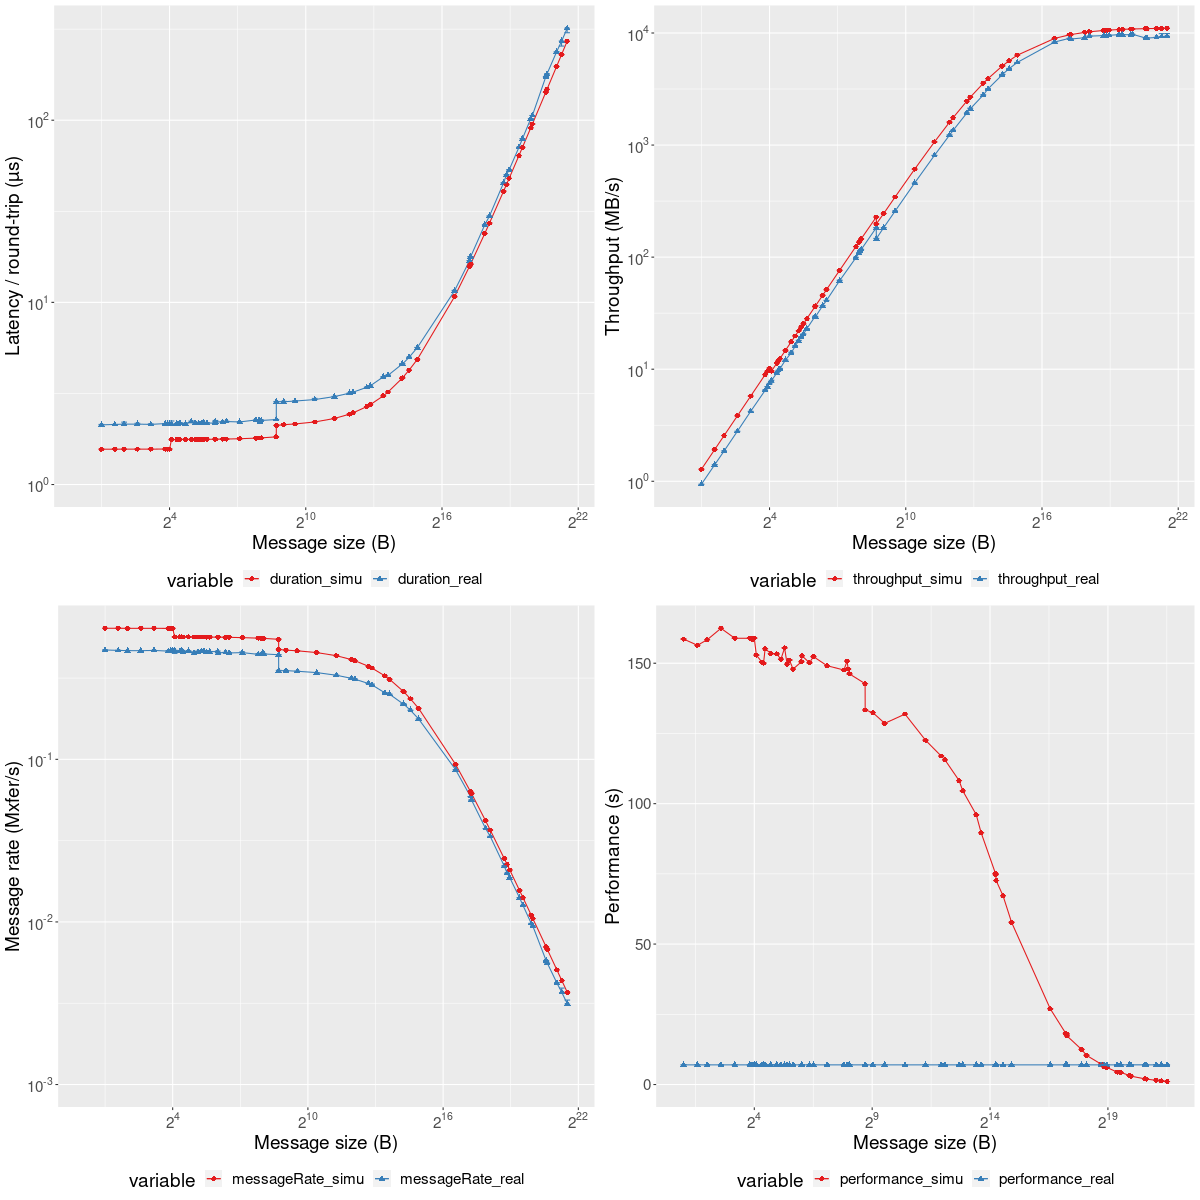
\includegraphics[width=\textwidth]{4_portals/ptlperf/ct.png}
    \caption{PtlPerf results for CT mode}
    \label{fig:4_portals:ptlperf_ct}
\end{figure}

\begin{figure}[!ht]
    \centering
    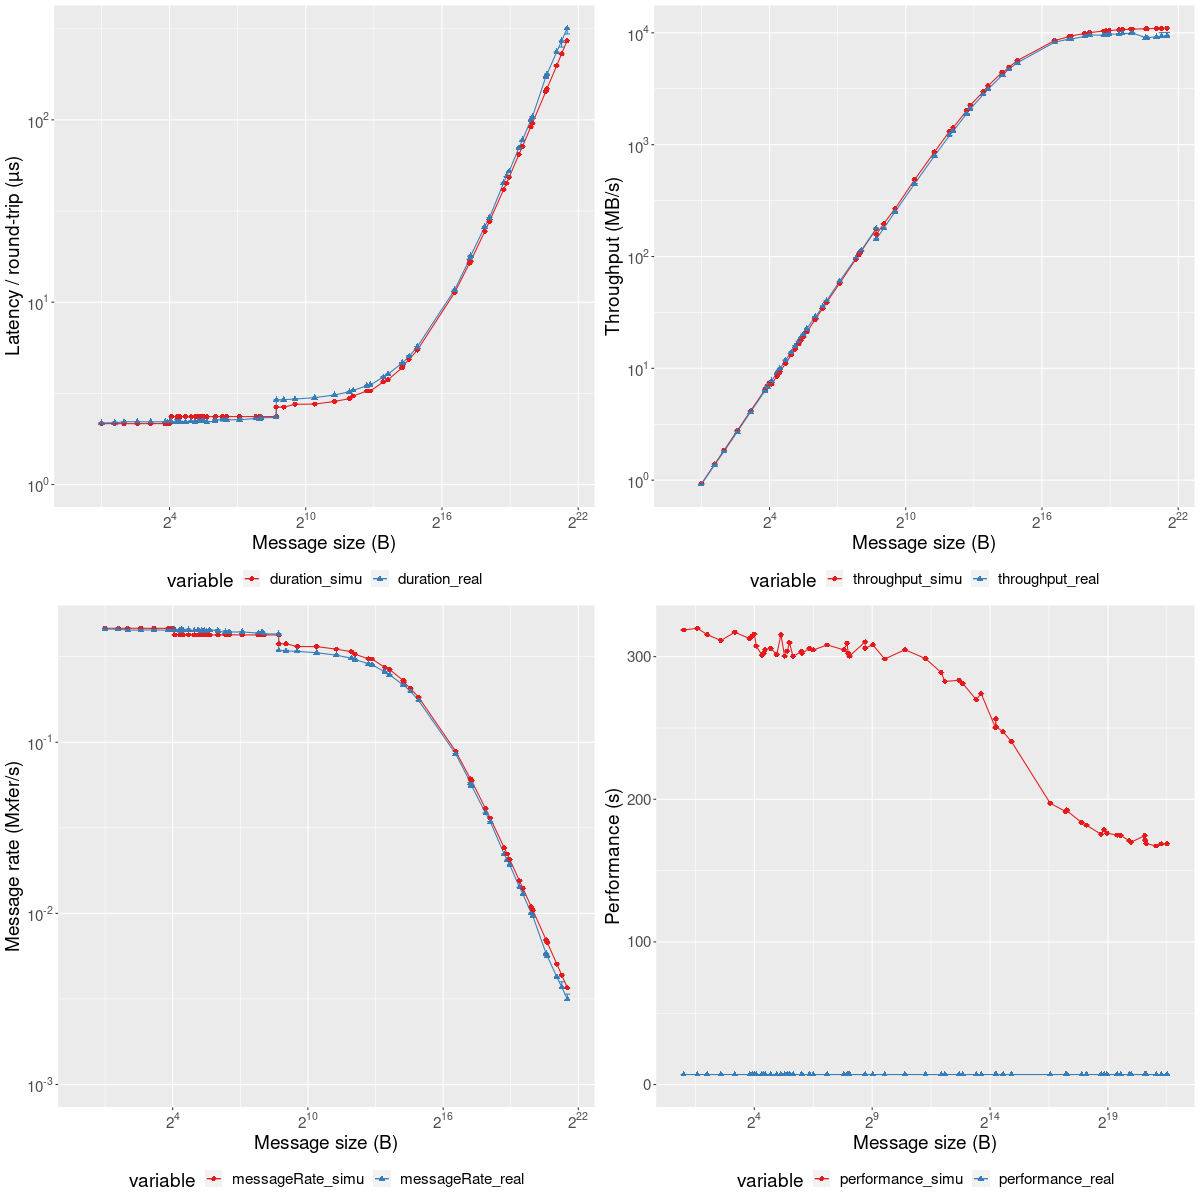
\includegraphics[width=\textwidth]{4_portals/ptlperf/ack.png}
    \caption{PtlPerf results for ACK mode}
    \label{fig:4_portals:ptlperf_ack}
\end{figure}

\begin{figure}[!p]
    \centering
    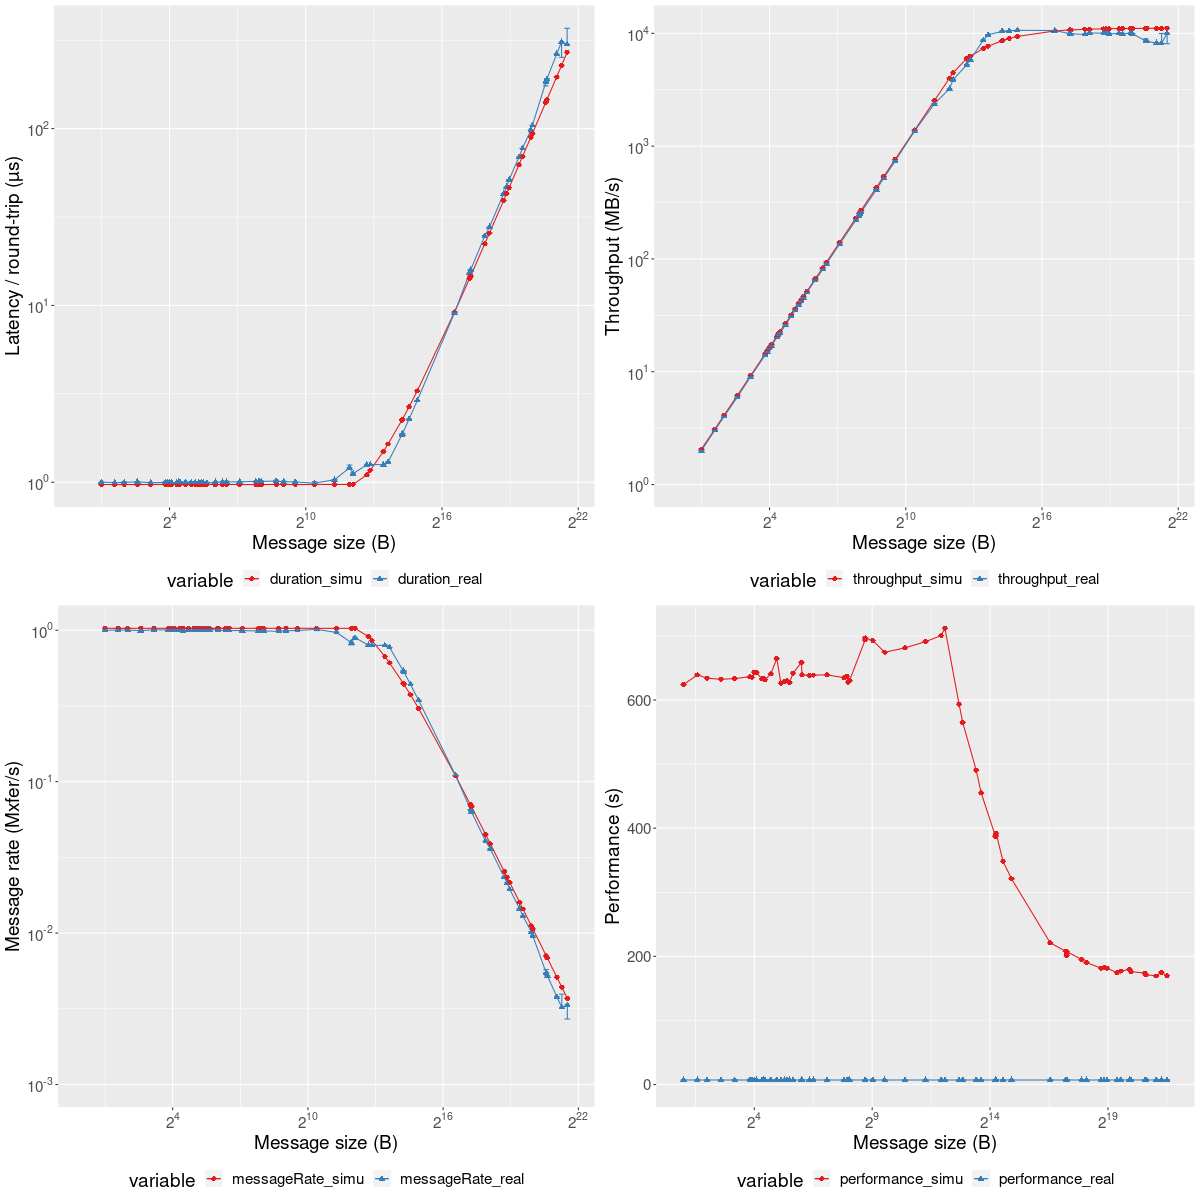
\includegraphics[width=\textwidth]{4_portals/ptlperf/match.png}
    \caption{PtlPerf results for match mode}
    \label{fig:4_portals:ptlperf_match}
\end{figure}

\begin{figure}[!p]
    \centering
    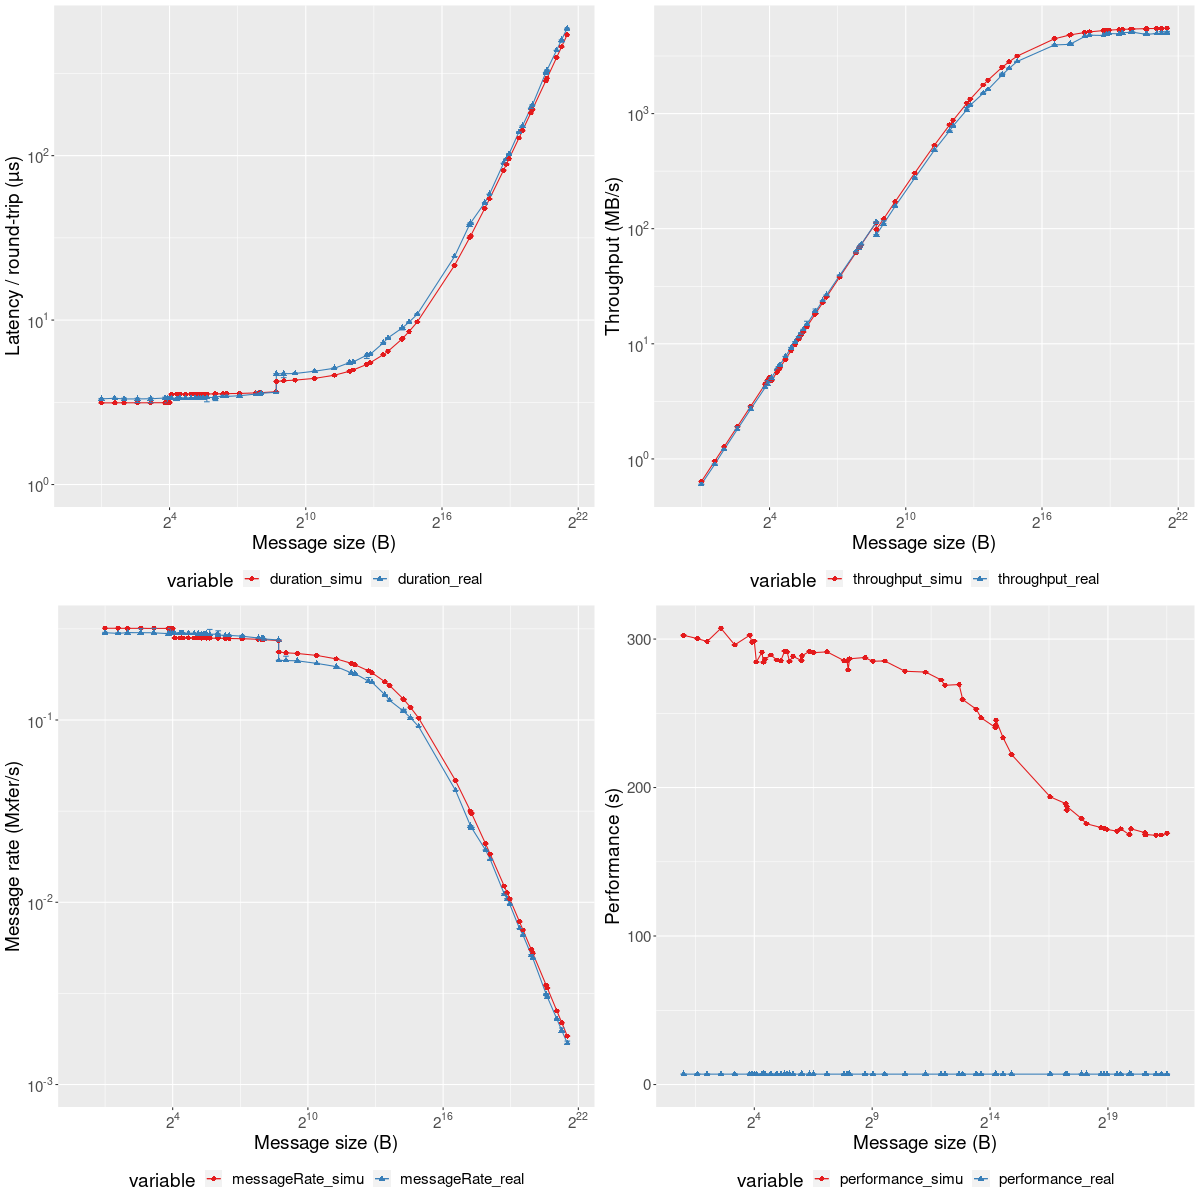
\includegraphics[width=\textwidth]{4_portals/ptlperf/reply.png}
    \caption{PtlPerf results for reply mode}
    \label{fig:4_portals:ptlperf_reply}
\end{figure}

Unlike our previous tests, which measure the time needed to send a fixed number
of messages, PtlPerf counts how many messages can be sent in a fixed amount of
time (using the \inline{PtlPut} primitive), and reports various statistics about the
transmissions (as presented in Section~\ref{subsubsec:2_context_hpc:ptlperf}).
While it offers many modes and options, we ran it in CT
(Figure~\ref{fig:4_portals:ptlperf_ct}), ACK
(Figure~\ref{fig:4_portals:ptlperf_ack}), match
(Figure~\ref{fig:4_portals:ptlperf_match}) and reply
(Figure~\ref{fig:4_portals:ptlperf_reply}) mode, for which the latency,
throughput, message rate, and performance of the simulator (in wallclock time)
compared to the real world execution are shown in the respective figures. CT,
ACK and reply mode all use one message inflight, as they are only meaningful in
this configuration, while for match mode we used the default limit on inflight
messages, which is 256.

We can see that ACK, match and reply modes have an excellent accuracy, and that
CT mode is acceptable even though it is not as perfect. From a performance point
of view, on all graphs we can see that larger messages cause the simulations to
be faster. This observation is expected, since in simulation no data is actually
transferred on a network, therefore modeling messages of all sizes has a similar
performance (no matter by how much the simulated time is increased, the
operation takes a constant amount of wall-clock time). Additionally, modeling
larger messages has an advantage for ptlperf in particular: since this benchmark
counts the number of messages sent in five seconds, instead of timing a fixed
number of iterations, it is expected that fewer operations will be performed
when larger messages are used, as each transfer takes more simulated time. 

We can also see that the performance of CT mode is much better than the other
ones, as it is the only benchmark which manages to be faster in simulation than
the real execution (for the biggest message sizes that we tested). The
explanation for this phenomenon comes from the way events are handled in
PtlPerf's code: after sending a message, the CT benchmark waits for the
completion of the communication using the \inline{PtlCTWait} primitive on a
counter. In simulation, this has the effect of putting the corresponding Actor
to sleep until the value of the counter is incremented, which is implemented in
an optimized way in our simulator. On the other hand, the other modes use full
events instead of counters, and instead of doing a \inline{PtlEQWait} in order
to wait for the completion of requests, they poll on the non-blocking
\inline{PtlEQGet} function between communications. In simulation, this has a
very negative effect on performance, because each polling loop only progresses
the simulated time by a very small amount, therefore the simulator will schedule
the polling Actor thousands of times before anything meaningful happens (like
receiving the event that is awaited), which is obviously very detrimental to
performance. This is a fundamental issue that is common in most Discrete Event
Simulators, and which we will discuss in more detail in the next chapter,
because we will see that it is particularly problematic in MPI (in
Section~\ref{subsec:5_high_level:polling}).
